%%
%% This is the 2018 To The Moon Burner Flight Manual
%%
%% Inspirational documents:
%% 
%% http://playadelfuego.org/sites/default/files/www_print_may13_web_spread.pdf
%% http://alchemyburn.com/sites/default/files/Alchemy-2015-Survival-Guide.pdf
%% http://www.euphoriaburn.com/sites/euphoriaburn.com/files/docs/Euphoria-2016-SurvivalGuide.pdf
%% https://drive.google.com/open?id=17P6mr4Ru1PN8U_qDDtwwpvcRyxrh4A0x
%% 

\documentclass[fontsize=11pt,paper=letter,titlepage,numbers=noenddot,final]{scrreprt}

% Failed experiment for smaller booklet size.  NOPE NOPE NOPE
%\documentclass[fontsize=10pt,paper=a5,titlepage,numbers=noenddot]{scrreprt}

% Ensure we expand to use more margin space
% Commented out as it seems to damage some of the section headers. Should be using KOMA scripts
% margin settings, anyway.
% \usepackage{fullpage}

% Type 1 fonts
\usepackage[T1]{fontenc}

% Include figures
\usepackage{graphicx}

% For SI Units; mostly to use for degrees.
\usepackage{siunitx}

% For nice slanted fractions
\usepackage{xfrac}

% For gobbling errant whitespace
\usepackage{xspace}

% Support for URLs and document links
\usepackage[hidelinks]{hyperref}
\hypersetup{colorlinks=false}

% for TODO items
\usepackage[usenames,dvipsnames]{xcolor}
\usepackage[disable]{todonotes}

% Fancy tables
\usepackage{booktabs}

% Allow for use of multiple columns
\usepackage{multicol}

% This provides a wee bit better typography
\usepackage{microtype}

% Make the labels for labeling lists look nicer with a sans serif font
\addtokomafont{labelinglabel}{\sffamily}

% This to grab the \square used in checklists
\usepackage{amssymb}

% Better lists
\usepackage{enumitem}

% Make a checklist environment
\newlist{checklist}{itemize}{2}
\setlist[checklist]{label=$\square$}

% \usepackage{libertine}
% \renewcommand{\familydefault}{\sfdefault}

% For better appendix support
% TODO Not sure if we want appendices; overkill?
\usepackage{appendix}

% sideways figures
\usepackage{rotating}

% figures wrapped in text
\usepackage{wrapfig}

% Glossary definitions and acronyms common to pre-flight manual and survival guide
%
% A list of glossary terms and acronyms
%
% Shared between pre-flight manual and survival guide
%

%%
%% Begin glossary stuff
%%
% \usepackage[acronym,style=long3colborder]{glossaries}
\usepackage[acronym]{glossaries}

\usepackage{glossary-longbooktabs}

% First use use full name of acronym, then the abbreviated.
\setacronymstyle{long-short}

% From https://en.wikibooks.org/wiki/LaTeX/Glossary#Defining_glossary_entries
% To support things that are both acronyms and glossary items, e.g., "MOOP."
\usepackage{xparse}
\DeclareDocumentCommand{\newdualentry}{ O{} O{} m m m m } {
  \newglossaryentry{gls-#3}{name={#5},text={#5\glsadd{#3}},
    description={#6},#1
  }
  \makeglossaries
  \newacronym[see={[Glossary:]{gls-#3}},#2]{#3}{#4}{#5\glsadd{gls-#3}}
}

% \makenoidxglossaries
\makeglossaries

% \newglossaryentry{moopgl}{
% name = {Matter Out of Place},
% description = {Anything not part of the natural environment, such as glitter, litter, bottle caps, and cigarette butts.}
% }

\newdualentry{moop} % label
  {MOOP}            % abbreviation
  {Matter Out of Place}  % long form
  {Trash, litter, things lost or left behind, things on the ground that should not be there.} % description
  

\newglossaryentry{rangers} {
name = {Rangers},
description = {A volunteer empowered to address safety concerns, mediate disputes, and resolve conflicts when they cannot be resolved by the persons involved}
% This is already in the team description for rangers
% \begin{labeling}{khaki}
% \item[alpha:] novice ranger
% \item[dirt:] (as in older than ...) an experienced ranger
% \item[khaki:] a Ranger that stays at HQ as a point-of-contact
% \end{labeling}}
}

\newglossaryentry{effigy} {
name = {effigy},
description = {The main art piece to be burned Saturday night.}
}

\newglossaryentry{graywater} {
name = {gray water},
description = {Water left-over from cleaning dishes or bathing.}
}

\newglossaryentry{crew} {
name = {crew},
description = {You.}
}

\newglossaryentry{gifting} {
name = {gifting},
description = {Giving food, an item, or a service without any expectation of reciprocity}
}

\newglossaryentry{mudburn} {
name = {Mud Burn},
description = {A burn characterized by extreme mud due to inclement weather}
}

\newglossaryentry{artcar} {
name = {Art Car},
description = {See: \gls{mutantvehicles}}
}

\newglossaryentry{mutantvehicles} {
name = {Mutant Vehicles},
description = {A motorized conveyance that is radically, stunningly, and safely modified. See also: \gls{artcar}}
}

\newglossaryentry{centercamp} {
name = {Center Camp},
description = {Host to many different musical experiences, performance art, and educational classes.}
}

\newglossaryentry{conclave} {
name = {Conclave},
description = {The Saturday night fire performance delivered by any interested and competent participants.}
}

\newglossaryentry{cockpit} {
name = {COCKpit},
description = {The main information station to visit when you have questions and need answers. There is also a huge map so you can find yourself. It's the home base for Volunteer Coordination, First Aid, \gls{lamplighters}, and \gls{lnt}}
}

\newglossaryentry{groundcontrol} {
name = {Ground Control},
description = {Department of Public Works Headquarters.}
}

\newglossaryentry{missioncontrol} {
name = {Mission Control},
description = {Rangers Headquarters.}
}

\newglossaryentry{shiftlead} {
name = {shift lead},
description = {some teams operator on a 24 $\times$ 7 schedule that is divided into shifts; a shift lead is one designated to be in charge of a given team for a shift}
}


\newglossaryentry{darkwad} {
name = {darkwad},
description = {Someone who is running around at night with no light or glow on. It gets dark out there. Real dark.}
}

\newglossaryentry{darksideofthemoon} {
name = {Dark Side of the Moon},
description = {Open camping located on the extreme eastern edge of the site well within the tree line.  Ideal for introverts without a theme camp, or those averse to the sun.}
}

\newglossaryentry{defaultworld} {
name = {default world},
description = {The rest of the world that is not a burn.}
}

% dual entry
\newdualentry{dmv} 
{DMV}
{Department of Mutant Vehicles}
{The volunteers who review and register \gls{mutantvehicles}, giving them permission to drive during the event.}


%dualentry
\newdualentry{dpw} 
{DPW}
{Department of Public Works}
{The team responsible for overseeing construction of the infrastructure, managing inventory, completing construction projects, overseeing Build Weekend and Tear Down, fueling the Effigy and Temple, and generally working behind the scenes during the event to deal with infrastructure issues as they arise. Also called Public Works.}

\newglossaryentry{education} {
name = {education},
description = {See: \glspl{greeter}}
}

\newglossaryentry{effigyburnfield} {
name = {Effigy Burn Field},
description = {This is where effigy and temple(s) get burnt.}
}

\newglossaryentry{eventleads} {
name = {event leads},
description = {This the team of volunteers who manage the event, and whom facilitate community needs. They are selected by the Board of Directors, which in turn is elected by the \gls{ttm} community.}
}

\newglossaryentry{gate} {
name = {Gate},
description = {The entrance to the burn where your ticket and ID will be checked, and where you will sign a waiver.}
}

\newglossaryentry{greeter} {
name = {Greeter},
description = {A friendly volunteer that will welcome you to the Burn, give you your \gls{swag}, and provide \gls{education} about the 10 (11) Principles. }
}

\newglossaryentry{groundscore} {
name = {ground score},
description = {\gls{moop} that is useful to you --- if you find something that someone dropped and you keep it, it's a ground score. If it looks valuable don’t be a dick, take it to lost and found. }
}

\newglossaryentry{lamplighters} {
name = {lamp lighters},
description = {The volunteer group that lights lanterns each night to illuminate some of the roads.}
}

\newglossaryentry{launchpad} {
name = {launchpad},
description = {Area where \gls{gate}/\glspl{greeter} are located.}
}

\newglossaryentry{temple} {
name = {temple},
description = {this is the art structure burned on the last night (though Euphoria has kindly donated their temple, which is to be burned Friday night)}
}

% dual entry
\newdualentry{lnt} 
{LNT}
{Leave No Trace}
{The concept that we should leave the property in better shape than we found it. It can also be verbed, as in ``Hey, I'm going to LNT the campsite after everyone packs up.'' }

\newglossaryentry{moonrangerstation} {
name = {Moon Ranger Station},
description = {Meeting point for Ranger Training.}
}

\newglossaryentry{opencamping} {
name = {open camping},
description = {where camping is permitted by participants who do not have a pre-assigned Theme Camp.}
}

\newglossaryentry{perimeter} {
name = {perimeter},
description = {Predetermined areas around the structure combustion events (Effigy, Temple, etc) that are staffed by volunteers to keep observers at a safe distance.}
}

% dual entry
\newdualentry{poop}
{POOP}
{Person Out of Place}
{People who are not where they should be. If you see someone passed out on the ground in the middle of the field, they may be drunk or having a medical emergency. Check and see if they are OK. If they want to be there, it's at their own risk if they get run over by a golf cart; but we try to get these people back to their camps.}

\newglossaryentry{sparklepony} {
name = {sparkle pony},
description = {A derogatory term for burners who show up to the event with little or no food or water, suitcases full of costumes and makeup, who do no work and no volunteering and only exist to look pretty, have fun, and party. They are often fashionably attired since they packed nothing but costumes.}
}

\newglossaryentry{swag} {
name = {swag},
description = {A memento from a burn, often wearable. You get swag for attending from \glspl{greeter}, often swag from your volunteer teams, and people you meet may gift you swag they made for the burn.}
}

\newglossaryentry{teamleads} {
name = {team leads},
description = {The people who head up each team that makes the burn happen.}
}

\newglossaryentry{tenprinciples} {
name = {Ten Principles},
description = {The ten core guiding concepts of most burns. }
}

\newglossaryentry{themecamp} {
name = {theme camp},
description = {A group of people camping together in a pre-assigned spot who often have common bonds and shared activities.}
}

\newglossaryentry{tbass} {
name = {Tranquility Base},
description = {(A.k.a., Tbase/Sanctuary) A dedicated space for those who may need an environment or area in which to better acclimate or adjust to the Burn.}
}

\newglossaryentry{village} {
name = {village},
description = {A group of Theme Camps sharing a common space and ethos.}
}

\newglossaryentry{eleventhprinciple} {
name = {11th Principle},
description = {The 11th Principle}
}


\newglossaryentry{preflightmanual} {
name = {pre-flight manual},
description = {The document that contains information essential for planning and preparing for \gls{ttm}}
}


\newglossaryentry{survivalguide} {
name = {survival guide},
description = {The document that contains information essential for planning and preparing for \gls{ttm}, and which provides information about events, theme camps, and art during the event.  Essentially, it is the \gls{preflightmanual} plus art, camp, and event listings.}
}


\newglossaryentry{parking} {
name = {Parking},
description = {There is a large parking area at the entrance.}
}

%% Glossary item template
% \newglossaryentry{} {
% name = {},
% sort = {},
% description = {}
% }

%% Glossary dual entry template -- i.e., things that are acronyms *and* glossary entries, like MOOP
% \newdualentry{OWD} % label
%   {OWD}            % abbreviation
%   {One-Way Delay}  % long form
%   {The time a packet uses through a network from one host to another} % description

\setglossarysection{subsection}


% acronym tag, short name, long name
\newacronym{ttm}   {TTM}      {To the Moon}
\newacronym{bod}   {BOD}      {Board of Directors}
\newacronym{leo}   {LEO}      {Law Enforcement Officer}
\newacronym{vc}    {VC}       {Volunteer Coordination}
\newacronym{gtfio} {GTFIO}    {Get the Fuck In and Out}
\newacronym{love}  {L.O.V.E.} {Lunar Orbit Vehicle Extraction}
\newacronym{pipo}  {PIPO}     {Pack in/pack out}
\newacronym{el}    {EL}       {Event Lead}
% \newacronym{SHORTNAME}  {ABBREV}  {LONGNAME}



%%
%% End glossary stuff
%%



% set text in a shape
\usepackage{shapepar}


\title{\textsf{To the Moon Burner's Pre-Flight Manual}}

\author{Piprrr, Raptor}


%%
%% For setting the title page background
%%
\usepackage{eso-pic}
\newcommand\BackgroundPic{%
\put(0,0){%
\parbox[b][\paperheight]{\paperwidth}{%
\vfill
\centering
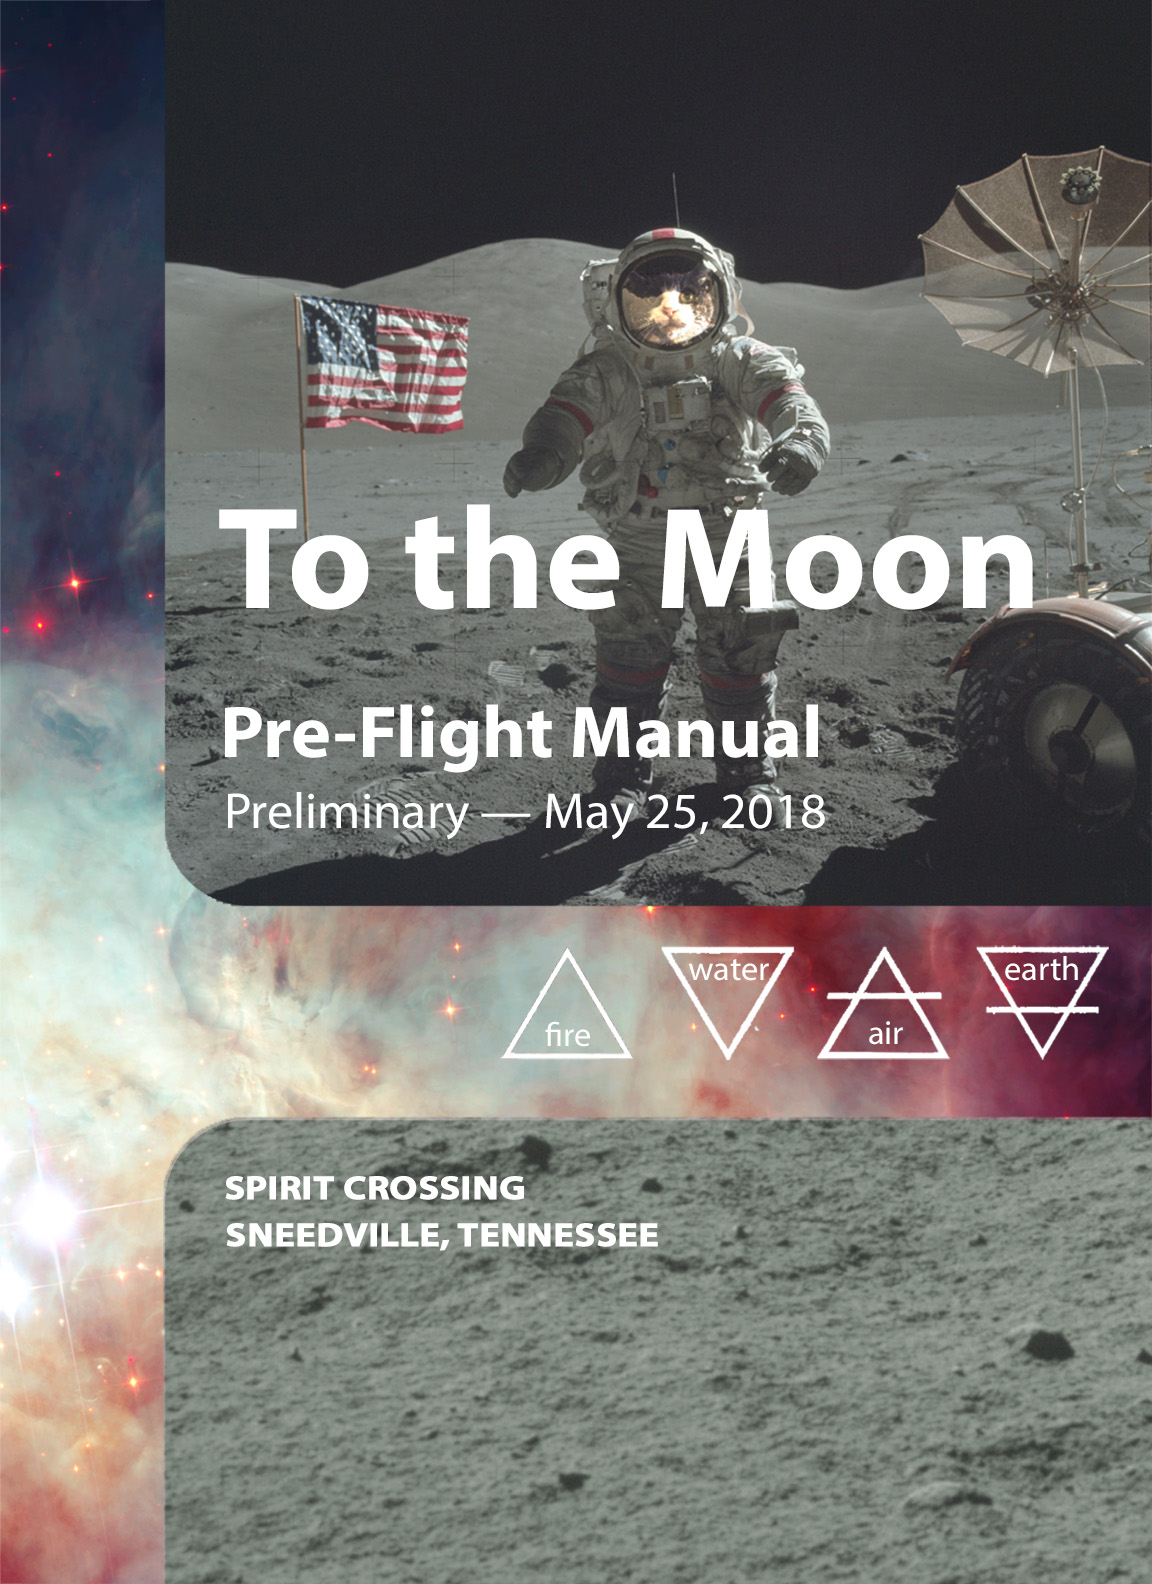
\includegraphics[width=\paperwidth,height=\paperheight]{images/coverpagePFM.jpg}%
\vfill
}}}

%% Remove leading space in new paragraphs
\setlength{\parindent}{0pt}
\setlength{\parskip}{.7em}
\widowpenalty 10000
\clubpenalty 10000

\newcommand{\bod}[2][]{\todo[color=green,#1]{#2}}

\begin{document}

\frenchspacing % eliminate extra spaces after periods

\begin{titlepage}
%% TODO Make title page similar to Apollo Flight Manual cover page
%% And now drop in the image for the title page
\AddToShipoutPicture*{\BackgroundPic}
\hspace{1em} %required to push the content of the next page out of this one
\end{titlepage}

% \maketitle not needed because we're using a titlepage environment
% \maketitle

\cleardoublepage

\tableofcontents

\pagestyle{headings}

\listoftodos

% include the introductory stuff
%
% This chapter provides history of TTM and gives the nod to volunteers and
% supporting organizations
%

\chapter[Welcome]{Welcome to the Moon, Traveler!!!}

% Welcome 

% What is To the Moon?
% History?
% This is true if only doing the flight manual, not the pre-flight
\ifisflight
  % This one page needs to be one column to look right, even
  % in the flight manual, proper.
  % failed experiment to add thumb guides
%   \addthumb{Welcome}{}{white}{black}
\putchapterthumb
\fi

\section*{Mission}
A Burn is a  multi day art and music camping event the intent of which is to build like minded community and to share:
your time, food, gifts, art, love, toys, and talents and participate in creating something in the process that inspires beyond measure.

"A unique and distinctive culture emerges from "The Burning Man" Experience. Rooted in the values expressed by the Ten Principles, this culture is manifested around the globe through art, communal effort, and innumerable individual acts of self expression. To many, it's a way of life." -Burning Man

\subsection*{To The Moon}
Burns reconnect one to their inner child and Merkabah, the divine light vehicle used to tune into the far realm of possibility and innovation.

Embark with us on a journey to the outer rims of creativity, art, music, and community as we initiate a collective experience geared towards positive transformation, endless inspiration, and participatory
co-creation. Bring your SELF, your talents, your radical self-expression, and your stardust TO THE MOON and back as we travel together further than our own imagination. You get out of it what you put int.

Simply put, we play with fire and run with scissors in a space shaped by our fantasy and that which is conjured up by our inspiration and elbow grease.... the sky is the limit. 

\subsection*{...And Back}
Art, Participation, Fire Play, Music and so much more motivate this 
community to build a temporary dwelling in which there is no stranger nor are there spectators. Everybody pitches in and brings something to the table.  
We stare at the clouds, dream in dust, set fire to the rain and howl at the moon.  

A Burn is an incredible way of learning firsthand the experience of the Whole being greater than the sum of its parts.  

It's a place where participants gather to celebrate self-expression and community who happen to know how to throw a party.  They conceive and build interactive theme camps, art installations, mutant vehicles, costumes and performances, and they gift them for the benefit and enjoyment of each other!

Art Camps, Theme Camps, Sounds Camps all are an integral part and at the heart of this experience.  The event comes to a climax with the burning of the Effigy Saturday night, and usually ends after Sunday's Temple Burn. 

The culture rallies around causes and activism from local art exhibits to food and coat drives to Burners Without Borders - spearheading change, inspiring involvement and making a splash! 

"In Dust we trust....."


\vspace*{\fill}
\begin{figure}[!h]
\centering
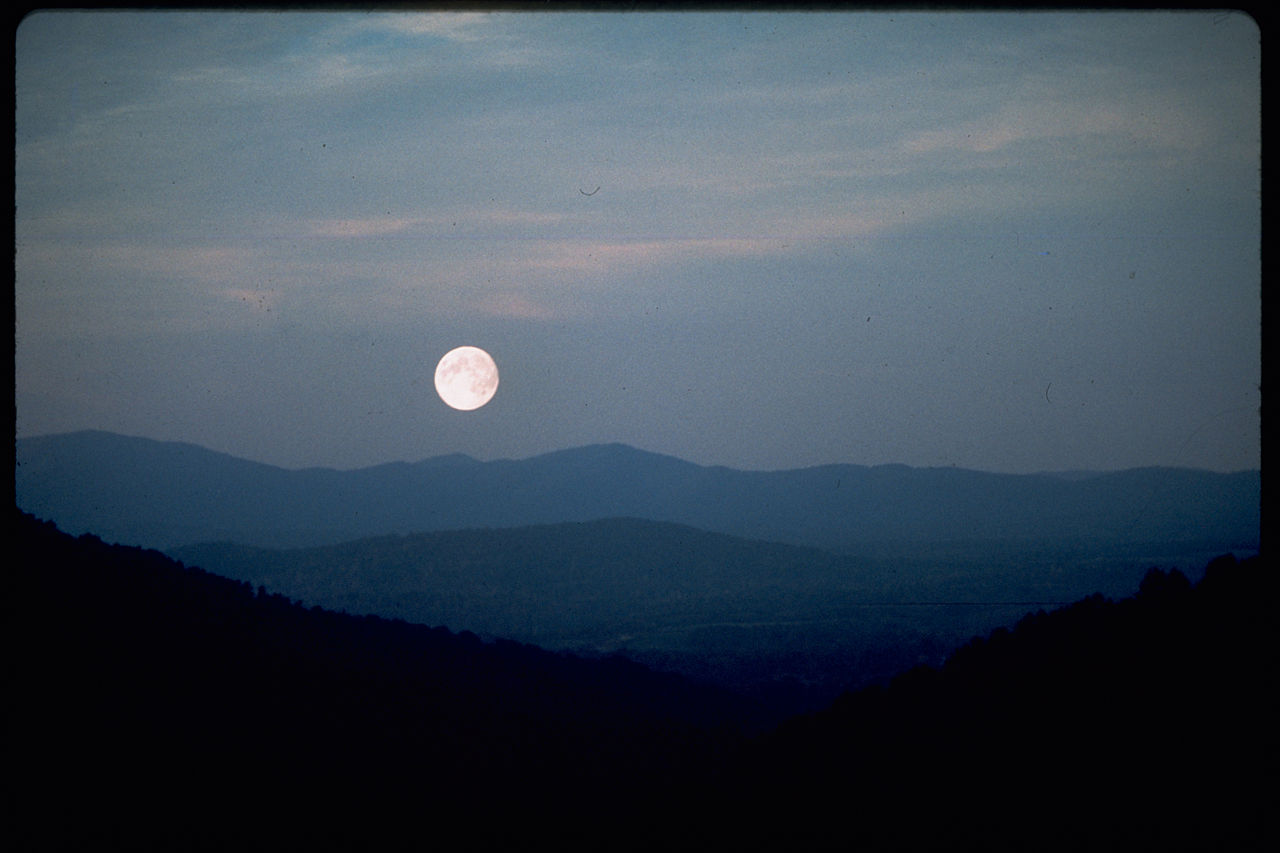
\includegraphics[width=.8\textwidth, trim=10 0 50 0, clip]{images/ShenandoahMoon}
% \caption{}
\label{image:mountainmoom}
\end{figure}
\vspace*{\fill}


% All things site, like directions, site maps, such as parking and (un)available amenities, checklist for packing
%
% Contains information about the site, such as directions, how to check-in, check-out, parking
% what services are available ... and not.  Stuff like that.
%

\chapter{Pre-Flight Procedures}

\section*{Find Us Online}

You can find us online at \url{https://www.tothemoonburn.com/}.  We also have a Facebook page at \href{https://www.facebook.com/groups/1686191044986642/?ref=bookmarks}{``To The Moon - An East TN River Burn''}.

\section*{Landing Site}

\begin{figure}[!h]
\centering
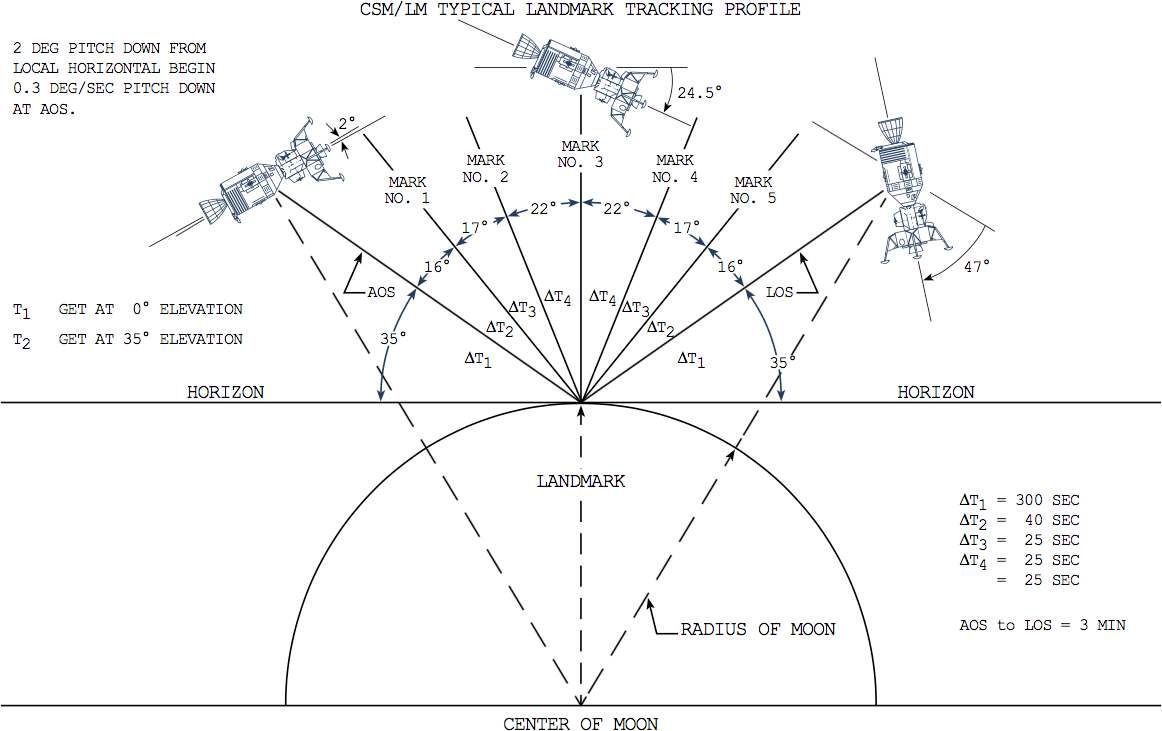
\includegraphics[width=0.9\textwidth]{images/landmarktracking.png}
% \caption{}
\label{image:landmarktracking}
\end{figure}

\begin{multicols}{3}

\subsection*{Landing Coordinates}
% \begin{quote}
36\si{\degree}31'59.0"N 83\si{\degree}08'57.0"W\\
\href{https://goo.gl/maps/pc3gYuNiF2r}{36.533051, -83.149169}
% \end{quote}

\subsection*{Address}
% \begin{quote}
Spirit Crossing\\
343 Clinch River Circle\\
Sneedville, Tennessee
% \end{quote}

\subsection*{Nearest Hospital}
% \begin{quote}
Hancock County Hospital\\
1519 Main St,\\
Sneedville, TN 37869
% \end{quote}

\end{multicols}

\begin{sidewaysfigure}[H]
\centering
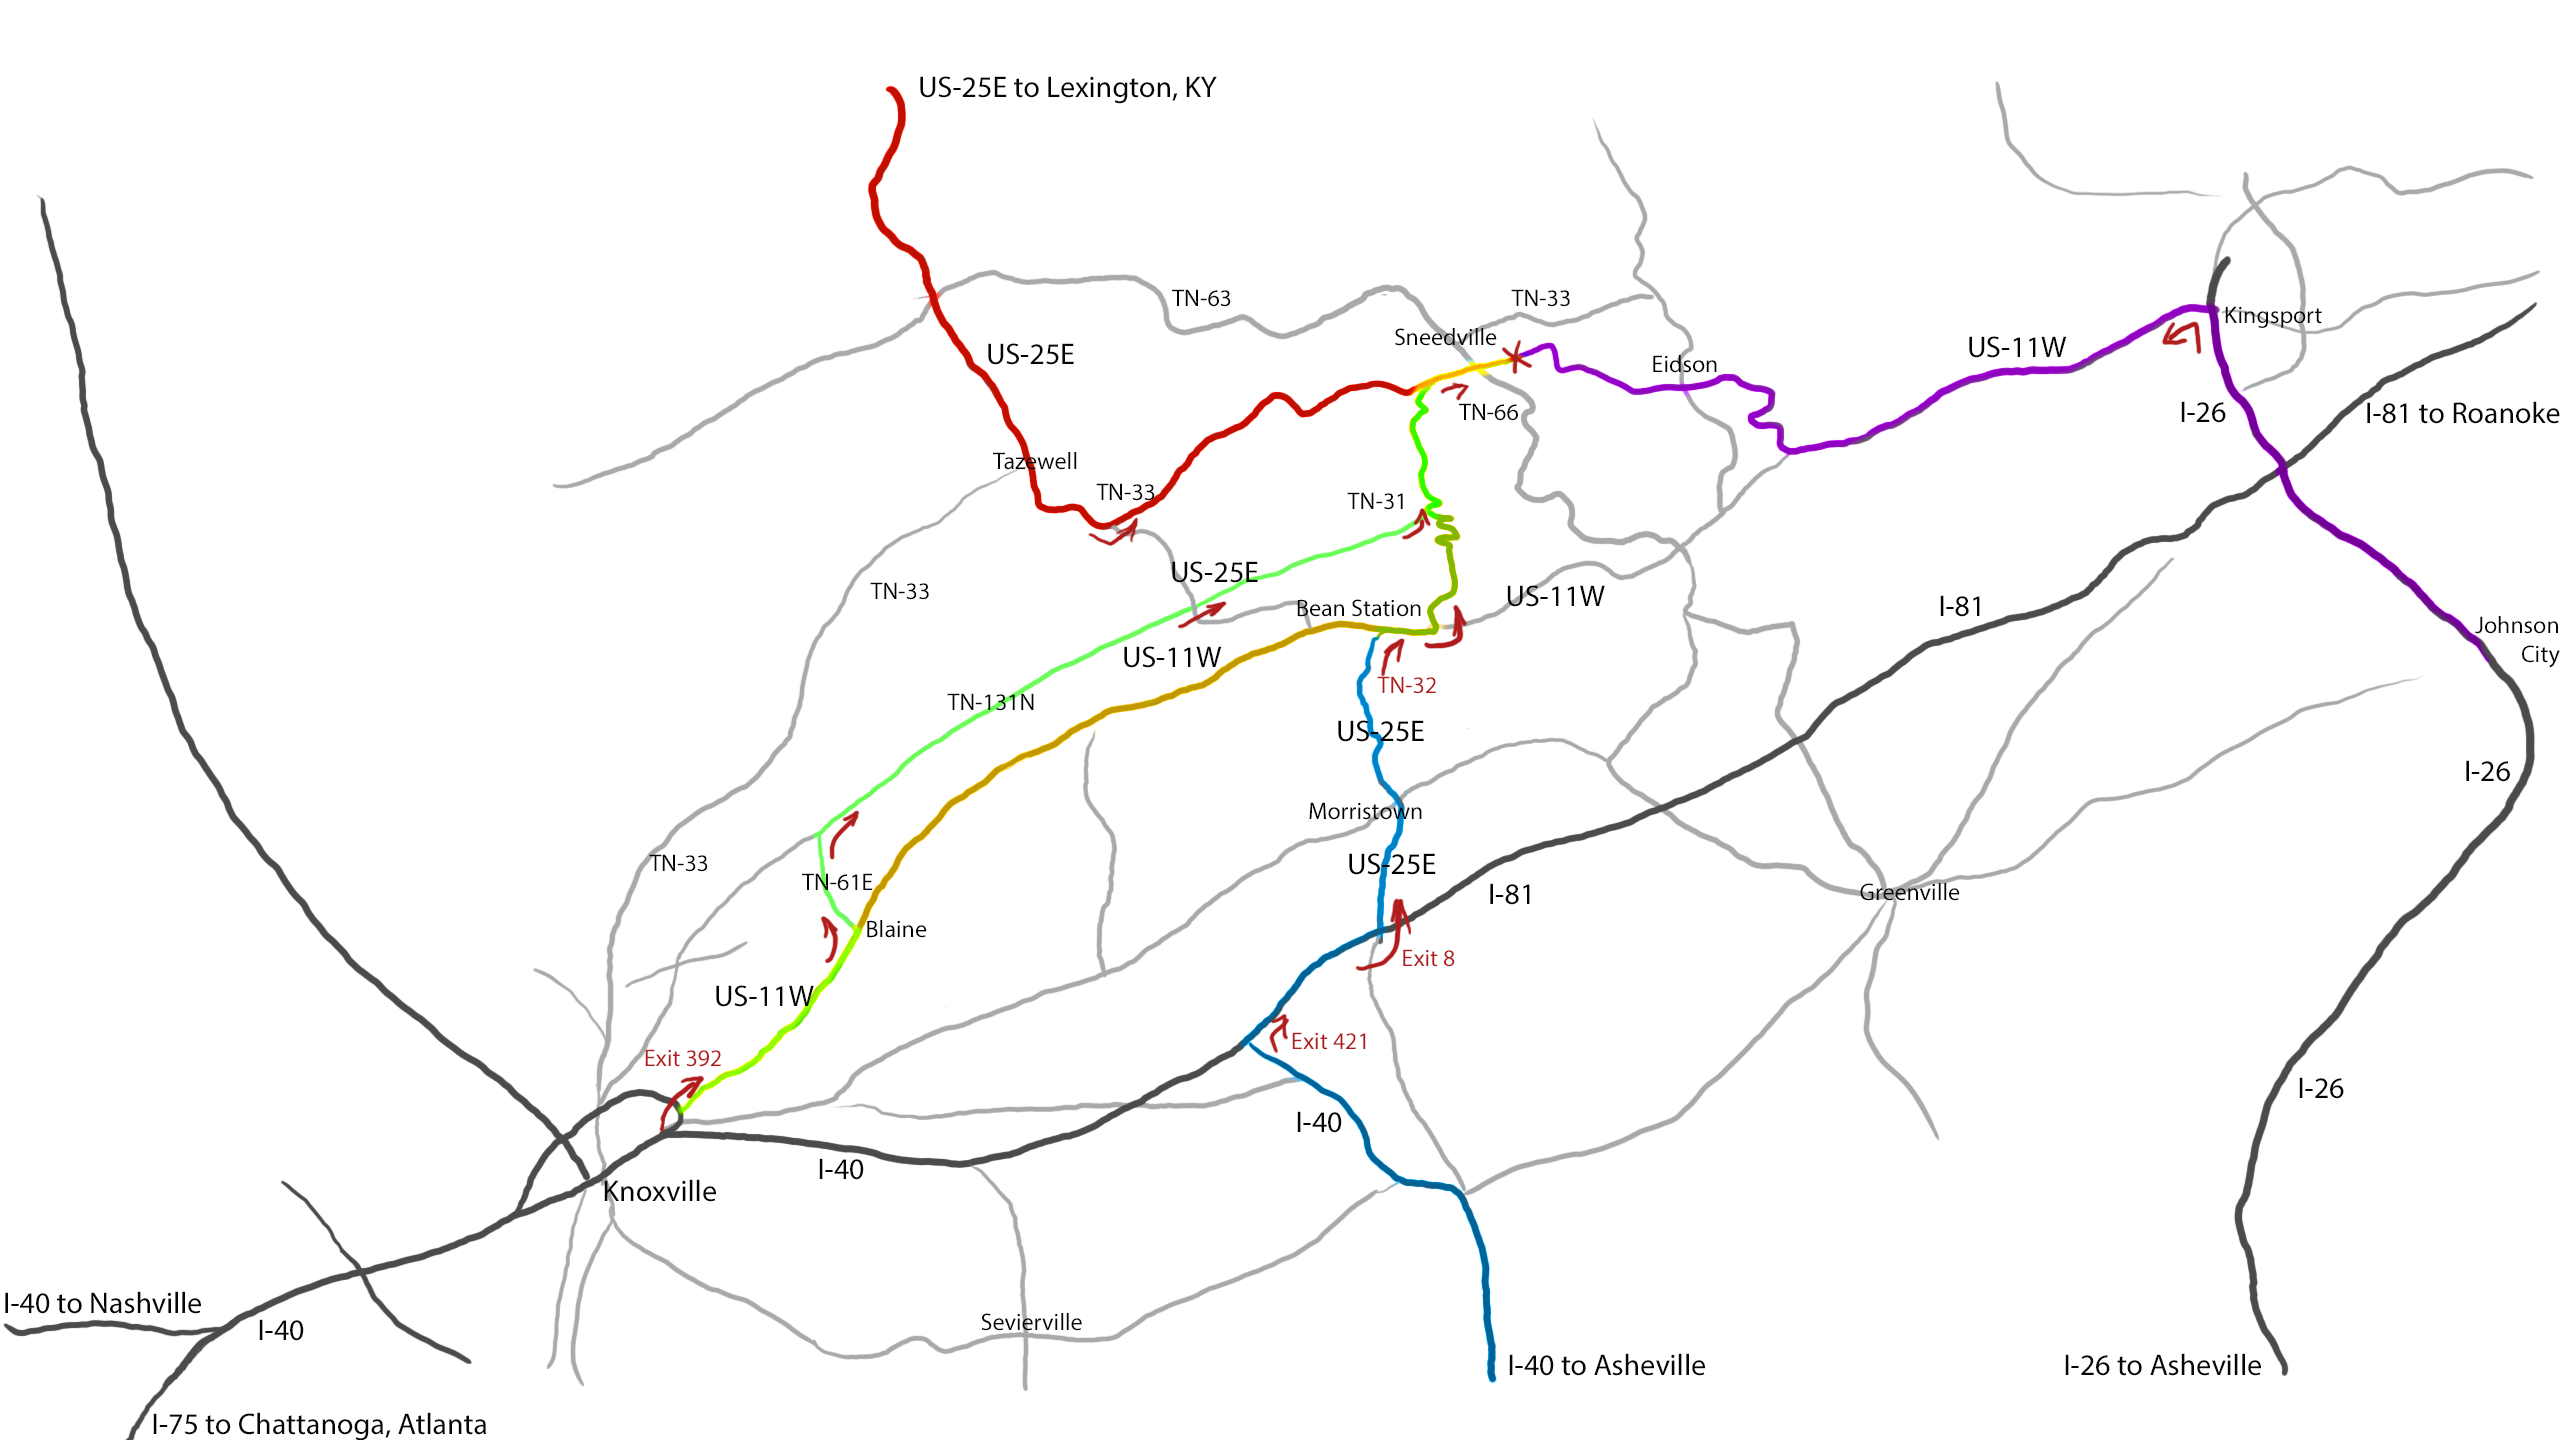
\includegraphics[width=\textwidth]{images/maptosite_highlighted.png}
\caption{Getting to the landing site. The colored-in routes are described in the following sections. Close-ups of the Bean Station and Sneedville areas can be found below.}
\label{image:overviewmap}
\end{sidewaysfigure}

\begin{figure}[H]
\centering
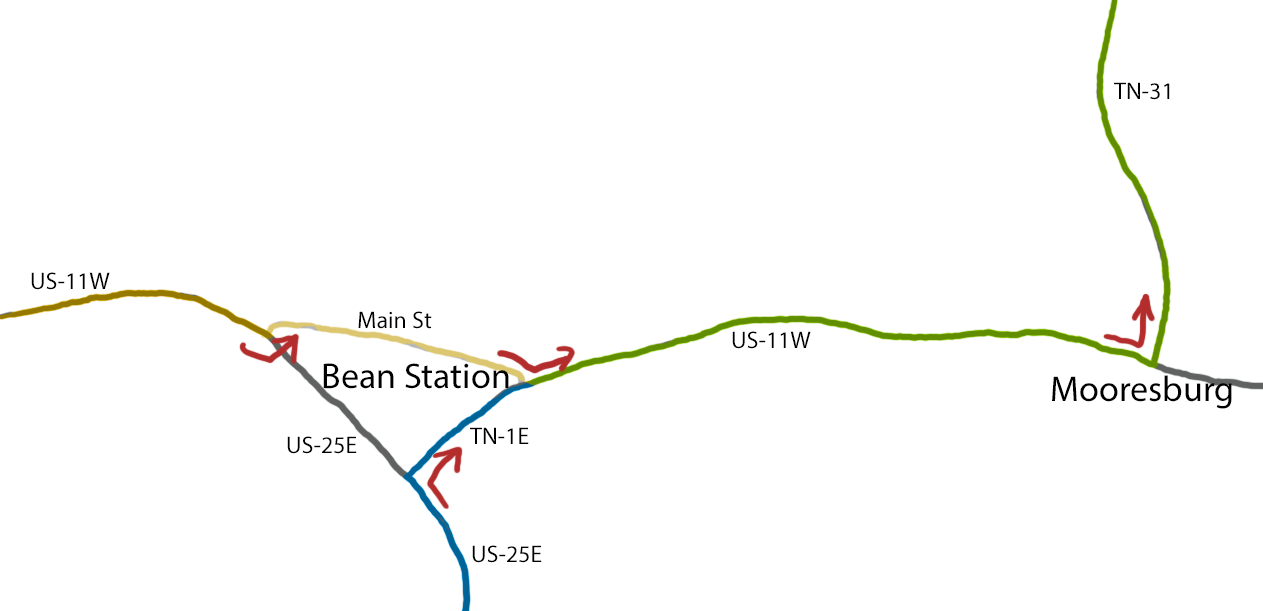
\includegraphics[width=.9\textwidth]{images/beanstationmap-highlighted.png}
\caption{Close-up of the Bean Station area. Crew from the Knoxville and Asheville direction will have to navigate this area.}
\label{image:beanstation}
\end{figure}
\vfill
\begin{figure}[H]
\centering
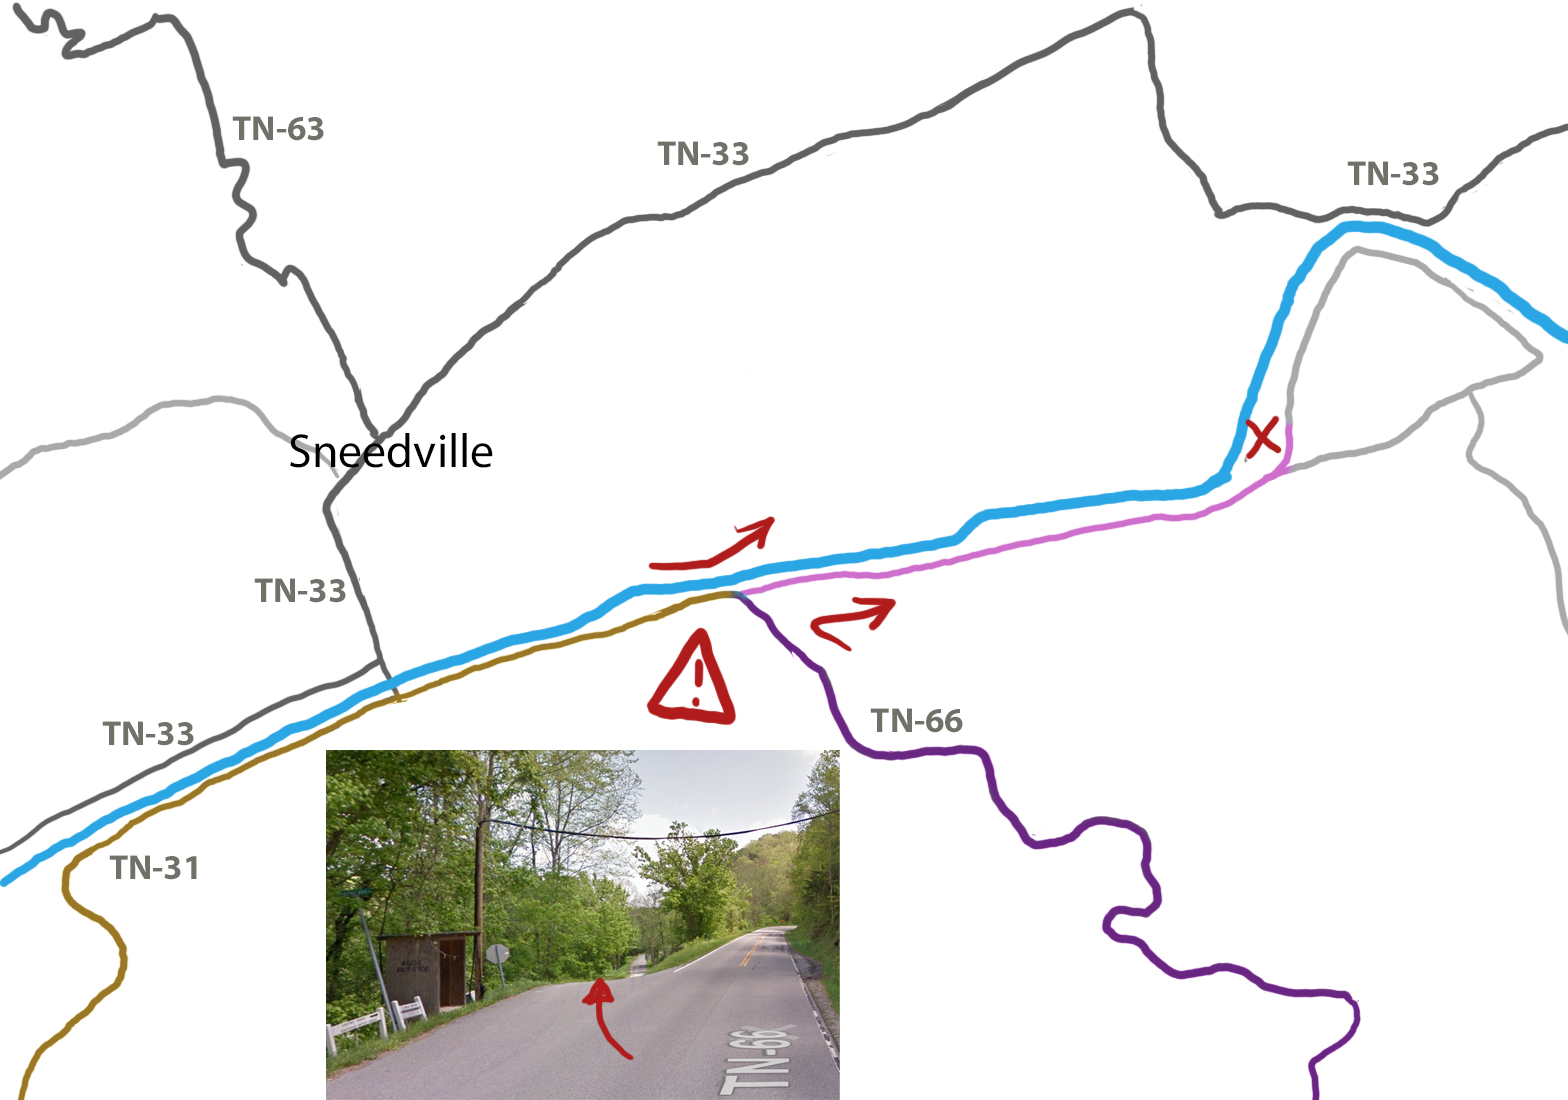
\includegraphics[width=.9\textwidth]{images/sneedville-closeup-highlighted.png}
\caption{Close-up of the Sneedville area and the Landing Site. Crew from all directions will have to navigate this area. Please pay special attention to the highlighted fork.}
\label{image:sneedville}
\end{figure}
% {\centering\label{image:overviewmap} 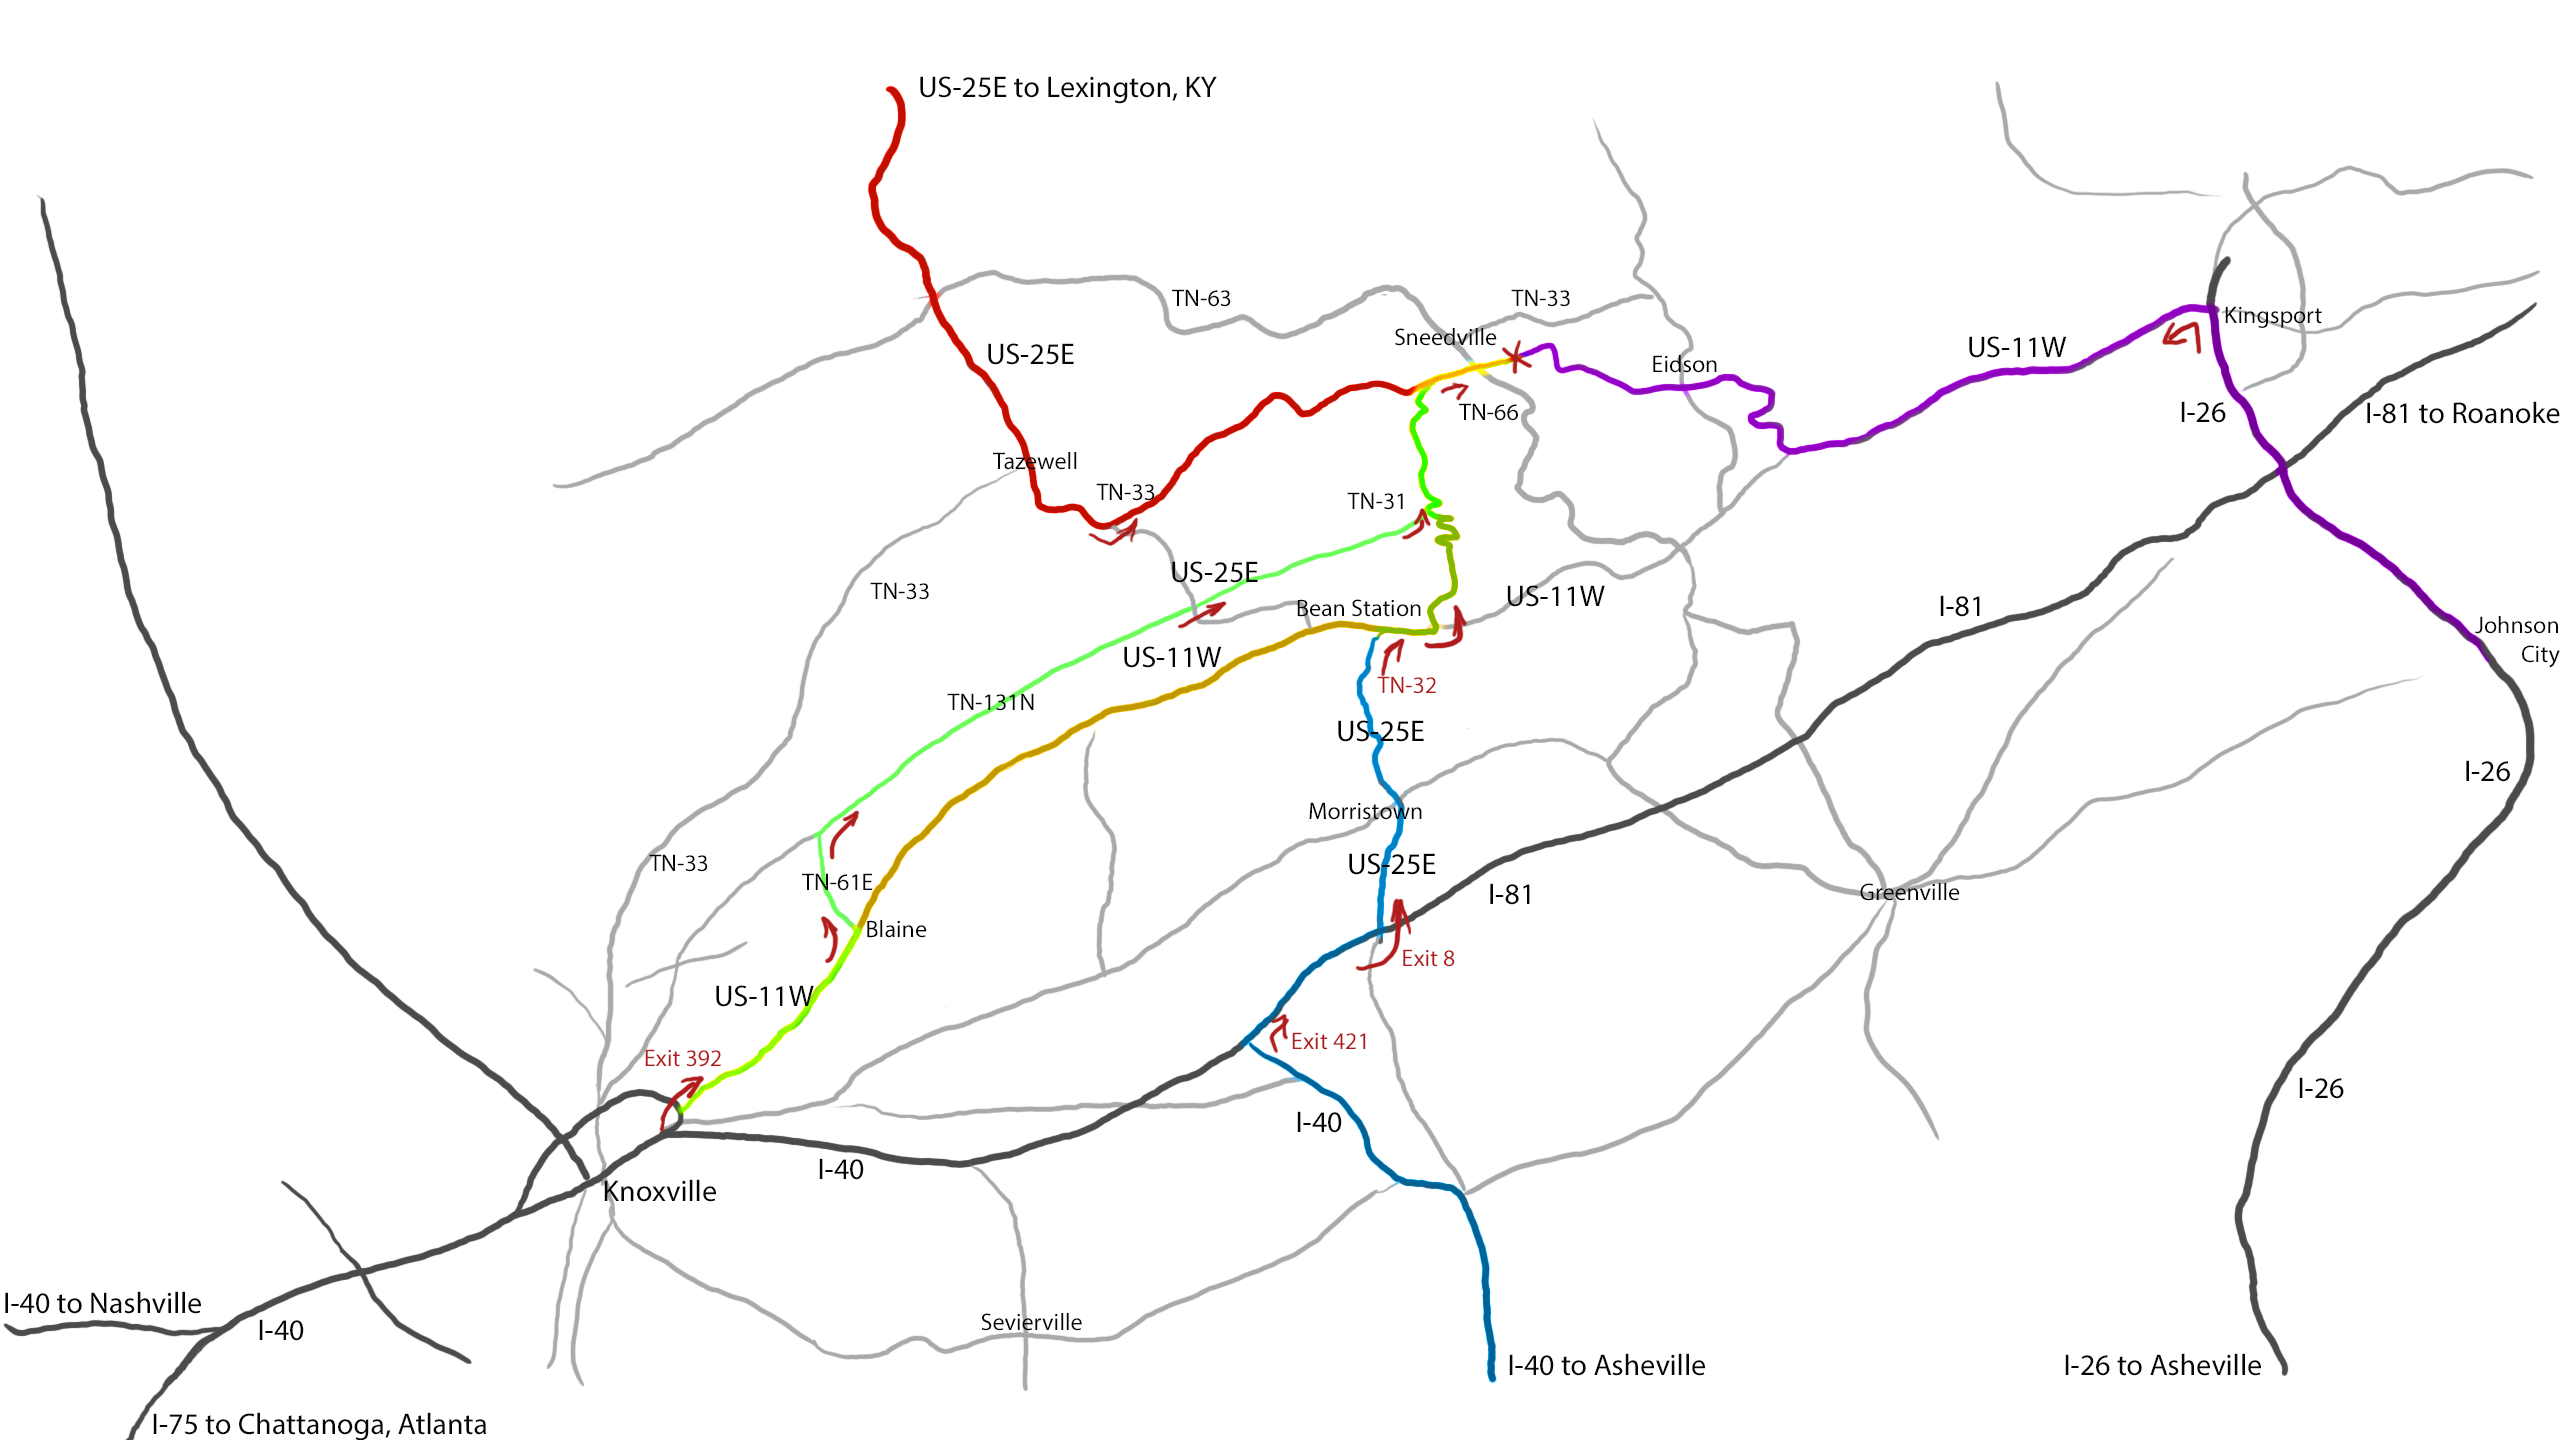
\includegraphics[height=\textheight]{images/maptosite_highlighted.png}}
% {\centering\label{image:beanstation}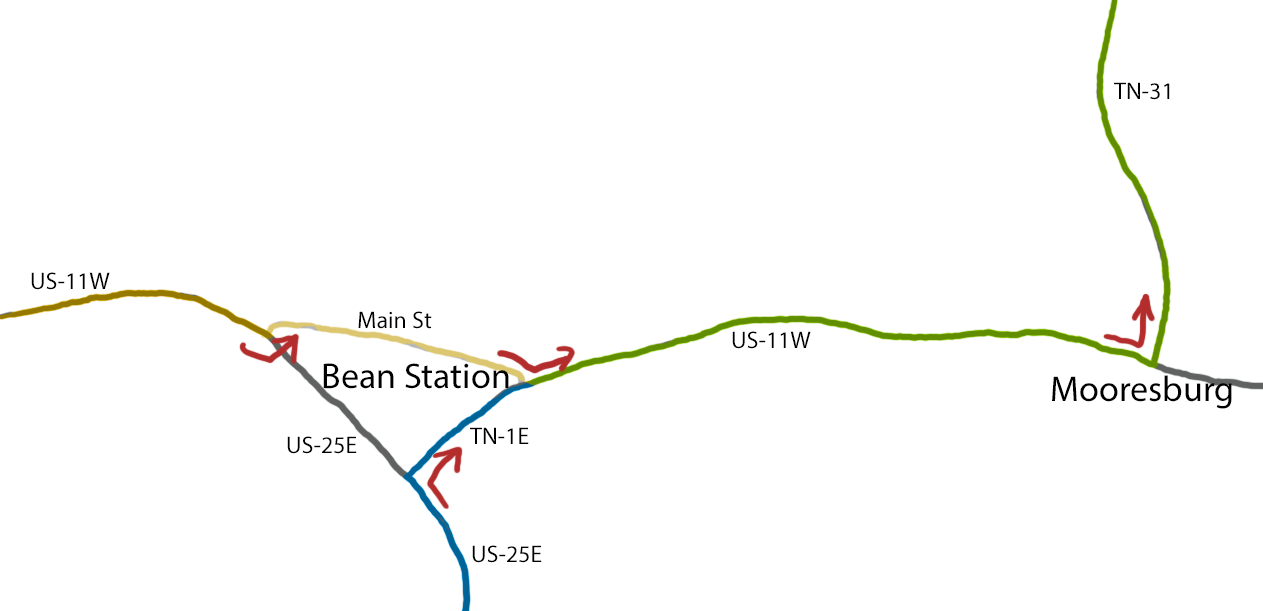
\includegraphics[width=\textwidth]{images/beanstationmap-highlighted.png}}
% \vfill
% {\centering\label{image:sneedville}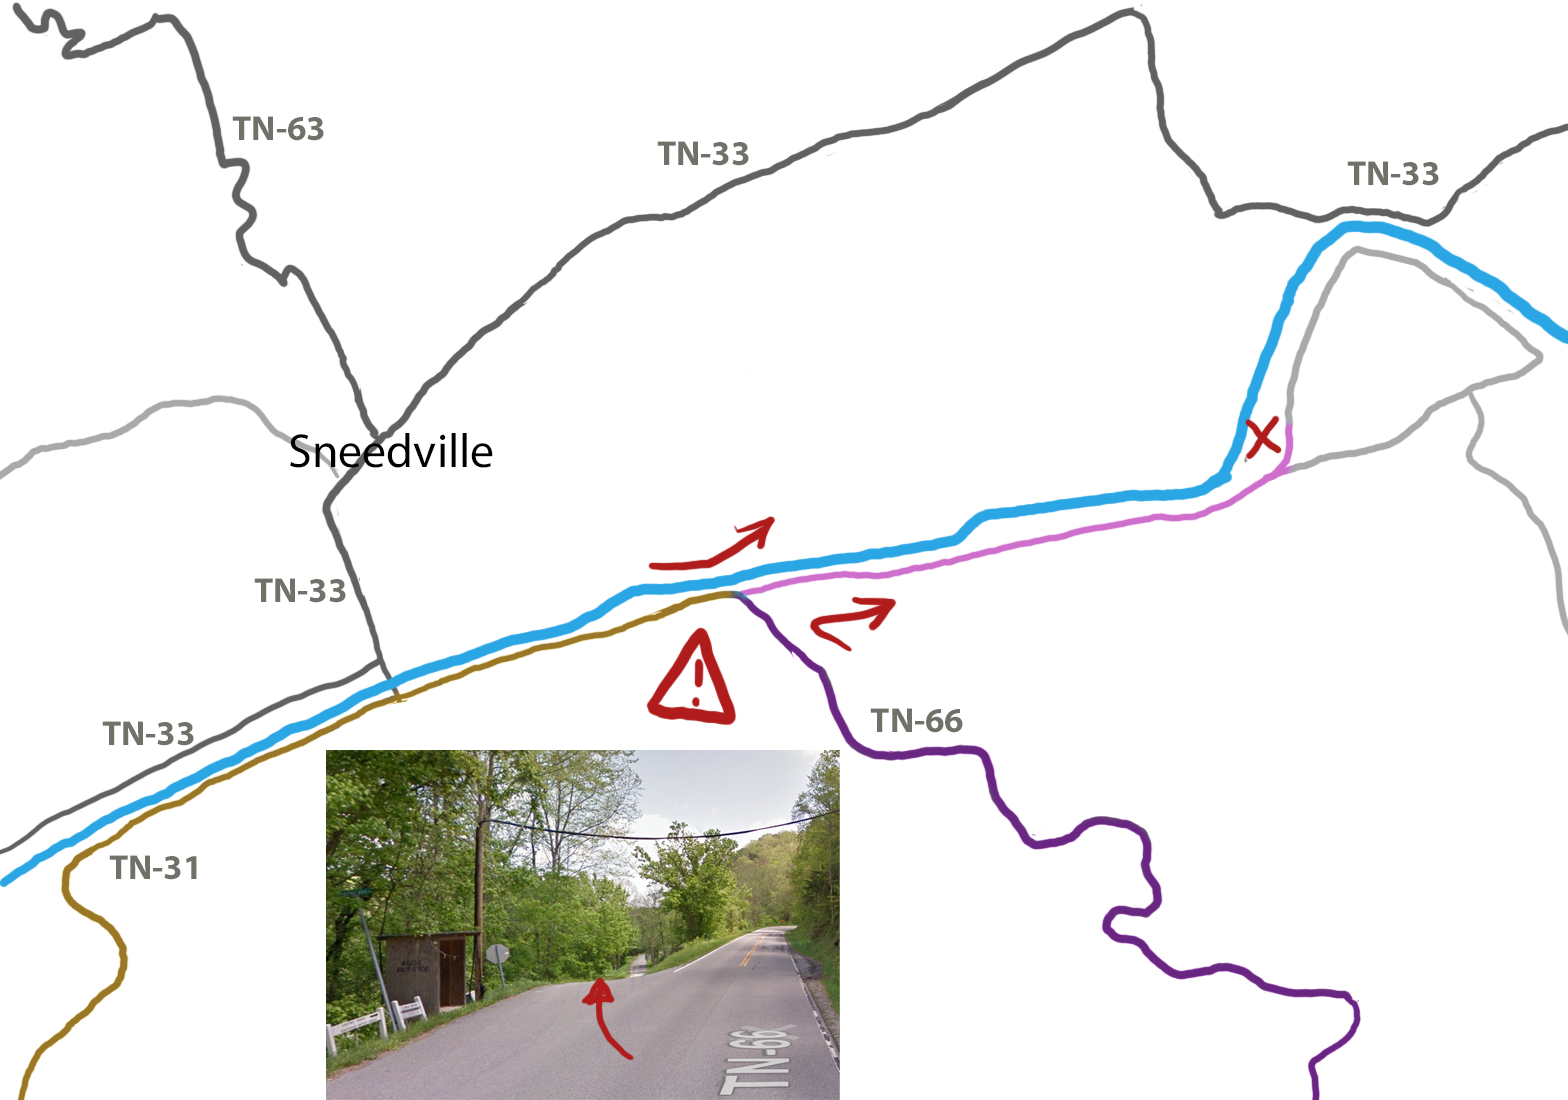
\includegraphics[width=\textwidth]{images/sneedville-closeup-highlighted.png}}

\subsection*{Flight Path}
A map of the flight path can be found on page \pageref{image:overviewmap}.
% \begin{wrapfigure}{R}{0.3\textwidth}
% \centering
% 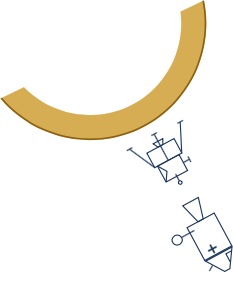
\includegraphics[width=0.25\textwidth]{images/landing1.png}
% % \caption{}
% \end{wrapfigure}


\subsubsection*{Struggle-Free Route (Green)}
The fastest routes to Spirit Crossing are full of switchbacks to avoid various objects in orbit. If you don't mind dodging the odd satellite, you can find instructions that suit your agile rocket needs. If your spaceship is rather large or you haul a shuttle, we recommend the struggle-free route. You can find this route on the maps highlighted in green.

\begin{enumerate}[noitemsep]
	\item Begin on I-40, headed towards exit 392 for US 11W N/Rutledge Pike/Knoxville Zoo.
	\item After 5.9 miles, turn left onto TN 61E. This road will turn into TN 131N.
    \item After about 16 miles you will pass through the small town of Washburn, in which the road takes a couple of wiggles left and right. Stay on the main road as you pass through. On your way out, you should pass a Dollar General on your left.
    \item Drive for about 23 miles, you will get to a stop sign. At this intersection, turn left onto TN 31N.
    \item Drive for another 9.7 miles, then take a slight left onto Chestnut Ridge Road. Continue from step \# \ref{dir:chestnutridge} in the ``From Knoxville'' directions.
\end{enumerate}

\subsubsection*{From Knoxville and points Southwest (Yellow)}
You can find this route on the maps highlighted in yellow.

\begin{enumerate}[noitemsep]
	\item Take I-40 E from downtown Knoxville.
    \item Take exit 392 for US 11W N/Rutledge Pike/Knoxville Zoo.
    \item Continue 40 miles to merge right onto US 11W / Hwy 25 E.
    \item After about a mile, turn left on to Main St.  You should see a red store on the left. A close-up of this area can be found on page \pageref{image:beanstation}.
    \item In about two miles, turn left on to US 11W.
    \item After about 2.8 miles, turn left on to TN 31.  There will be an Exxon station on the left at the intersection. \label{dir:tn31}
    \item Drive for about 17 miles and then continue straight on to TN 66 S.
    \item Drive 1.4 miles for slight left onto Chestnut Ridge Road.  Look for the ``To the Moon'' sign along the road; \textbf{this is a tricky intersection that's easy to miss. \label{dir:chestnutridge} You can find a picture and close-up of this area in the Sneedville area map on page \pageref{image:sneedville}}
    \item After about \sfrac{1}{3} of a mile, turn left on to Clinch River Circle
    \item Welcome home!  Please follow instructions in the next section, ``Landing Procedure,'' on page \pageref{sec:parking}
\end{enumerate}


\clearpage
\subsubsection*{From Asheville and points Southeast (Blue)}
You can find this route on the maps highlighted in blue.

\begin{enumerate}[noitemsep]
	\item Take I-40 W to I-81
    \item Take exit 8 for US 25 E towards Morristown/White Pine
    \item Take exit to 11W north towards Rogersville
    \item In Bean Station, continue on TN-1 E/TN-32 N. A close-up of this area can be found on page \pageref{image:beanstation}.
    \item Continue from step \# \ref{dir:tn31} in the ``From Knoxville'' directions
\end{enumerate}


\subsubsection*{From Johnson City and points East (Dark Pink)}
You can find this route on the maps highlighted in dark pink.

\begin{enumerate}[noitemsep]
	\item Take I-26W
    \item Continue on US23 through Kingsport
    \item Turn left on VA 600/VA 623
    \item Continue straight on VA-696
    \item Continue on TN-33 S
    \item Turn left on TN-70 S
    \item Turn right on Chestnut Ridge Road. This is a steep turn! You can find a picture and close-up of this area in the Sneedville area map on page \pageref{image:sneedville}
    \item Turn right on Clinch River Circle
    \item Welcome home!  Please follow instructions in the next section, ``Landing Procedure,'' on page \pageref{sec:parking}
\end{enumerate}


\subsubsection*{From Lexington, KY and points North (Red)}
You can find this route on the maps highlighted in red.

\begin{enumerate}[noitemsep]
	\item Take I-75 S
    \item Take exit 29 for US-25E, turn left onto US-25E
    \item Turn left onto TN-33 N
    \item Turn right onto TN-31 S/TN-66 S
    \item Turn left onto TN-66 S
    \item Resume from step \# \ref{dir:chestnutridge} in the ``From Knoxville'' directions
\end{enumerate}

\section*{\Gls{gate} Hours}
\label{sec:gate}

Please see Table \ref{tbl:gatehours} on page \pageref{tbl:gatehours} for a detailed list of gate hours.

\Gls{gate} is closed during and after Effigy and Temple Burn

\textbf{** No admission after 6 p.m. Saturday **}
 
All unused tickets are void after 6pm Saturday and the burn is closed for entry. 

\textbf{** Absolutely no ticket sales at the gate **}

\clearpage

\section*{Landing Procedure}
\label{sec:parking}

% \bod[inline]{This will have to be vetted and expanded by gate and/or BoD}

\begin{enumerate}[noitemsep]
	\item arrive at Spirit Crossing entrance where \gls{parking} volunteers will navigate you to a staging area for check-in
    \item check-in at \gls{gate} with tickets and ID
    \item receive wrist-band; keep this wrist-band with you at all times (please see page \pageref{sub:wristbands} for more information on wristband policy)
    \item proceed to \glspl{greeter} to be properly welcomed and oriented -- be sure to get your swag!
 	\item offload equipment at your deployment site
      \begin{itemize}
          \item If you are driving an RV or using a camper
              \begin{quote}
                  \gls{parking} will direct you to your final deployment area for RVs and campers
              \end{quote}
          \item If you are driving a regular vehicle
              \begin{itemize}
          		\item If this is a \gls{mudburn}
              		\begin{quote}
              			if the site is too muddy for vehicles, you may have to hoof in your gear; or, coordinate with the \gls{gate} on asking \gls{love} to shuttle your gear to your site
              		\end{quote}
          		\item If the grounds are driveable
              		\begin{enumerate}
                       \item Since there is limited access on-site for bringing vehicles for offloading coordinate with \gls{gate} for getting an offloading pass 
                       \item drive to site
                       \item offload gear (do NOT take the time to set up!)
                       \item drive back to \gls{gate} to return offload pass
                    \end{enumerate}
                \item If you arrive after dark (regardless of weather conditions), \gls{love} will shuttle participants' belongings from the \gls{gate} to their camps, eliminating the presence of burner blinding non-art cars freely roaming the burn field.
             \end{itemize}
      \end{itemize}
    \item return to \gls{parking} to properly land vehicle for event duration
    \item finish deploying your gear at your camping site
%      \item go to \gls{parking} to land vehicle into assigned landing pad
%     \item check-in with \gls{gate} that you have offloaded
\end{enumerate}

\begin{table}[h!]
\centering
\caption{\Gls{ttm} \gls{gate} hours}
\label{tbl:gatehours}
\begin{tabular}{@{}lll@{}}
\toprule
Wednesday & 6/13/2018 & 12--10\pm EST                                    \\ 
          &           & Theme Camp Early Entry Only w/ Pre-Registration \\
Thursday  & 6/14/2018 & 10\am--12\am EST                                   \\
Friday    & 6/15/2018 & 10\am--10\pm EST, for people                                   \\
          &           & 10\am--8\pm EST, for vehicles\\
Saturday  & 6/16/2018 & 10\am--6\pm EST                                    \\
          &           & No admission after 6pm for rest of event        \\
Sunday    & 6/17/2018 & 10\am--6\pm EST                                    \\
          &           & Departing Only                                  \\
Monday    & 6/18/2018 & 8\am--12\pm EST                                    \\
          &           & Departing Only                                  \\ \bottomrule
\end{tabular}
\end{table}
\textbf{No vehicles will be allowed in after sunset! No moving vehicles \textit{period} inside the burn when it's dark - so if you get there right before sunset, you better get in, unload your stuff, and get right back out to parking ASAP. This is for the safety of everyone at the burn!}

Any vehicles that arrive after sunset will be redirected to parking, where we may or may not have a golf cart to help you carry some stuff in --- but don't count on it --- use that Radical Self-Reliance!

\section*{Re-entry Procedure}

\textbf{There is no after hours entry without pre-arranged permission.  Crew arriving at the site outside gate operating hours will be turned away.  No crew is permitted to wait on the property until the gate opens.}

Please contact the \gls{bod} via \url{connect@tothemooonburn.com} well in advance of the event to work out options if long-distance travelers cannot arrive while the gate is open.

For the safety of other patrons and to preserve the integrity of the experience, \textbf{no} coming and going at leisure is allowed after checking in.  Exiting and returning \gls{ttm} are reserved \textbf{for medical and emergency reasons only}, and must be communicated to and cleared by the Gate Lead prior to leaving.

Theme Camp supply runs are possible Wednesday -- Friday before 10\pm \textbf{only}. Before leaving, \textbf{check at the gate} if a pass is needed. The Gate will check with \Gls{el} on call and a re-entry lanyard will be issued at \gls{el} discretion.

% If you forget something and need to ``make a run to the store'' talk to a team / event  / gate lead and we can grant Re-Entry if you combine your trip with one beneficial \gls{ttm} and the community at large.

\section*{Takeoff Procedure}
\subsection*{Leave No Trace}
\Gls{ttm} follows the \gls{lnt} principle (see \gls{tenprinciples}, page \pageref{tenprinciples}). Please take all your belongings, trash, and \gls{graywater} with you and leave the site in a better shape than you found it.

\subsection*{Takeoff Launch Window}

\Gls{ttm} officially closes at 11:59\pm EST, Sunday, June 17th.  All crew must vacate the site by 12pm EST, Monday, June 18th unless given explicit prior permission from Theme Camp Late Departure.

Vehicles can be driven on site on Monday to pack up. In case of inclement weather, a no driving / limited access policy to site will be implemented. Be prepared by bringing your own cart / wagon to transport gear out and to your vehicle.
\Gls{love} will be able to assist with shuttling gear to parking. 
Vehicles can \textbf{not} be parked alongside road to do so, but only be lined up at gate about 10 at a time.

Pleases look for announcements at \Gls{cockpit} / \Gls{gate}, as this policy may slightly change, depending on situation. 

% \begin{figure}
% 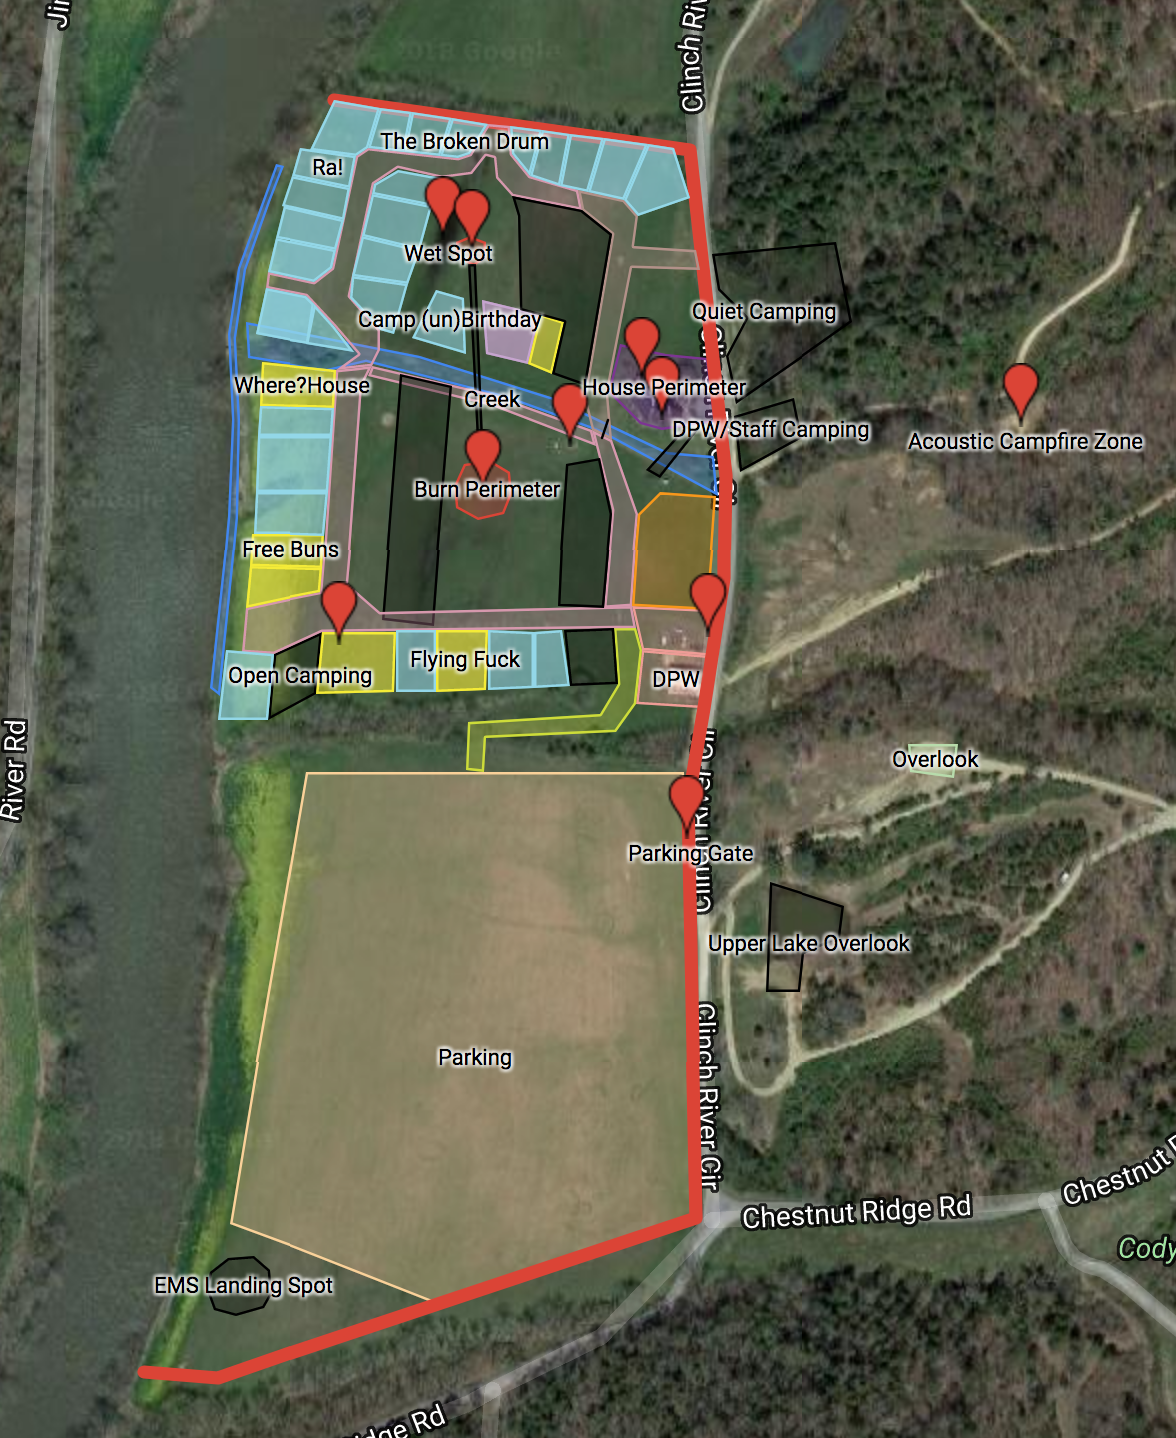
\includegraphics[width=.8\textwidth]{images/sitemap-placeholder.png}
% \caption{2017 version; needs updating. Map of the landing site. Need updated version, properly styled, etc.}
% \label{image:sitemap}
% \end{figure}


% \section{Where to camp}
% \missingfigure{Site map highlighting approved camping areas }

% \section{Crew Restricted Areas}
% \missingfigure{Site map highlighting public vs crew only areas}


% \section{Pre-flight Procedures}
\section*{Crew Equipment}
% Things to do / pack before leaving
\gls{ttm} is an exercise in radical self-reliance.  This means bringing everything you are going to need, which includes food, water, shelter, any medications, and hygiene products.  You must take responsibility for your own well-being and survival.  Do not expect the community to take care of you.  Though there are EMTs on site, they are only an emergency resource, so do not rely on them for basic over-the-counter medications.

\subsection*{Crew Inventory Checklist}
Below is a list of items we suggest you bring with you.  A burn requires a certain amount of preparation to be able to sustain you for 4--5 days of camping with minimal amenities. Please come prepared.  While this isn't the Playa, the nearest store is a bit removed so pack what you need and extra.  

% The following are checklists for items that are recommended to bring to ensure maximum likelihood of survival and an otherwise hoopilicious time.  The first checklist is for items that crew should bring; the second are for nice to have items.

\subsubsection*{Must Haves}

\begin{multicols}{2}

\begin{checklist}
	\item \textbf{A valid, state-issued} photo ID
    \item Your printed ticket
    \item Emergency contact
    \item 1 gallon of water per person per day!  Spirit Crossing does not provide water but does have a well accessible if needed - bring your own. In case of shortage, a hose is available for filling up but please plan ahead!
\end{checklist}
\end{multicols}

\subsubsection*{Strongly Recommended}

\begin{multicols}{2}

\begin{checklist}
	\item tent
    \item sleeping bag and/or bedding
    \item blankets
    \item tarps
    \item 3 gallons of water per person per day for drinking, washing, and food preparation
    \item food for everyone in your group for length of stay
    \item any necessary medication
    \item epi pen
    \item if needed, contact lens supplies
    \item first aid kit
    \item sunblock
    \item insect repellent
    \item single ply toilet paper \footnote{The port-a-potties only get serviced once a day, and may run out of toilet paper.}
    \item garbage bags, recycling bags, and tools for \gls{moop} containment
    \item flashlights, spare batteries, headlamps, LEDs for your camp  (solar powered recommended) 
    \item sunglasses
    \item reusable cup or bottle \footnote{Many camps offer drinks, but do not provide cups.  A cup with a carabiner is ideal.}
    \item reusable utensils and dinnerware \footnote{Many camps offer food, but do not provide utensils or plates}
    \item towels
    \item sufficient ice for duration \footnote{Some stores also sell dry ice. However, be sure to wrap dry ice in towel for further insulation.}
    \item deodorant
    \item paper towels
    \item biodegradeable dishwashing soap \footnote{Do not wash dishes in the river, and exercise proper gray water management.}
    \item biodegradeable body washing soap \footnote{Please do not wash in the river.}
    \item condoms
    \item pocket knife
    \item hammer
    \item baby wipes or moist towelettes
    \item rain hat / rain gear / umbrellas
    \item \gls{graywater} container and funnel \footnote{A cat litter bucket works well as gray water containment.}
    \item gifts
    \item a loving and open mind
    \item \hrulefill
\end{checklist}

% * <mcoletti@gmail.com> 2018-05-08T17:10:50.436Z:
% 
% >     \item \hrulefill
% Possibly add more of these to fill out the page.
% 
% ^.
\todo[inline]{reorder a bit to keep topics together?}

\end{multicols}

\subsubsection*{Optional}

\begin{multicols}{2}

\begin{checklist}
    \item swimsuit
    \item water shoes
    \item inner-tube
    \item can or bottle opener
    \item portable metal ashtrays \footnote{Mint tins work well for this purpose.}
    \item lawn chairs
    \item pop-up shelters, pavilions, or other forms of portable shelter
    \item ice chests
    \item camp cooking stove
    \item fuel for stove 
    \item earplugs
    \item watertight protective bags \footnote{For cameras and electronics.}
    \item rope, string, zip ties, duct tape
	\item spray bottle of water for keeping cool
    \item generator
    \item simple toolkit
    \item sewing kit
    \item rubber mallet
    \item tea and/or coffee
    \item musical instruments
    \item coffee pot, tea pot, or french press
    \item parasols
    \item fire bowl
    \item fire wood
    \item pasties
    \item fire extinguishers
    \item fuel and safety gear for fire performance 
\end{checklist}

\end{multicols}


\subsection*{Prohibited Items} %\todo{themed name?}
Please do not bring \textbf{any} of the following items:

\begin{multicols}{2}
\begin{itemize}[noitemsep]
	\item Handheld lasers --- they are too powerful to be safe
    \item Fireworks --- unsafe use of fire and creates \gls{moop}
    \item Chinese/fire lanterns --- uncontrollable, flaming \gls{moop} 
    \item Pets of any kind (please see pets policy on page \pageref{sub:nopets})
\end{itemize}
\end{multicols}

\clearpage
\section*{Resources}

% \begin{wrapfigure}{R}{0.3\textwidth}[h!]
% \centering
% 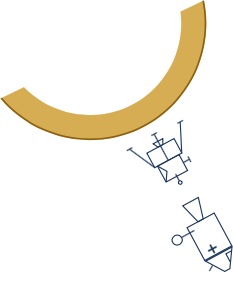
\includegraphics[width=0.25\textwidth]{images/landing1.png}
% % \caption{}
% \end{wrapfigure}
\begin{multicols}{2}
\subsection*{Showers}
There are no showers. To keep yourself clean, bring wet wipes or biodegradable soap.
Please don't clean your dishes or yourself in the river since there are mussels in the river that are protected wildlife.  (And these are also the reason you should wear river shoes while in the river as the mussels will cut you.  They're mean that way.)

\subsection*{Food}
There will be no food vendors. Bring plenty of food for yourself and to share (see \gls{gifting}, page \pageref{gifting}).

\subsection*{Ice}
Ice is available twice a day for \$2 per 10 lbs bag.  Cash only! Bring small bills please. 
Times tbd. Sorry, no presales --- yet.

\subsection*{Lost and Found}
The Lost and Found will be at the \gls{cockpit} / \gls{vc} station.

\subsection*{Port-a-Potties}
There are Port-a-Potties on-site. Please don't put anything other than one-ply toilet paper and human waste in the Port-a-Potties. You will find Port-a-Potties in multiple locations across the site.



\vspace{1em}
\reflectbox{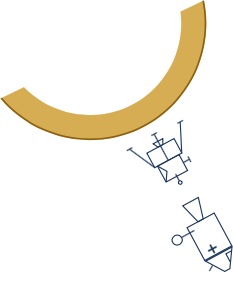
\includegraphics[width=\columnwidth,angle=180]{images/landing1.png}}
\end{multicols}

% \vspace{3cm}
% 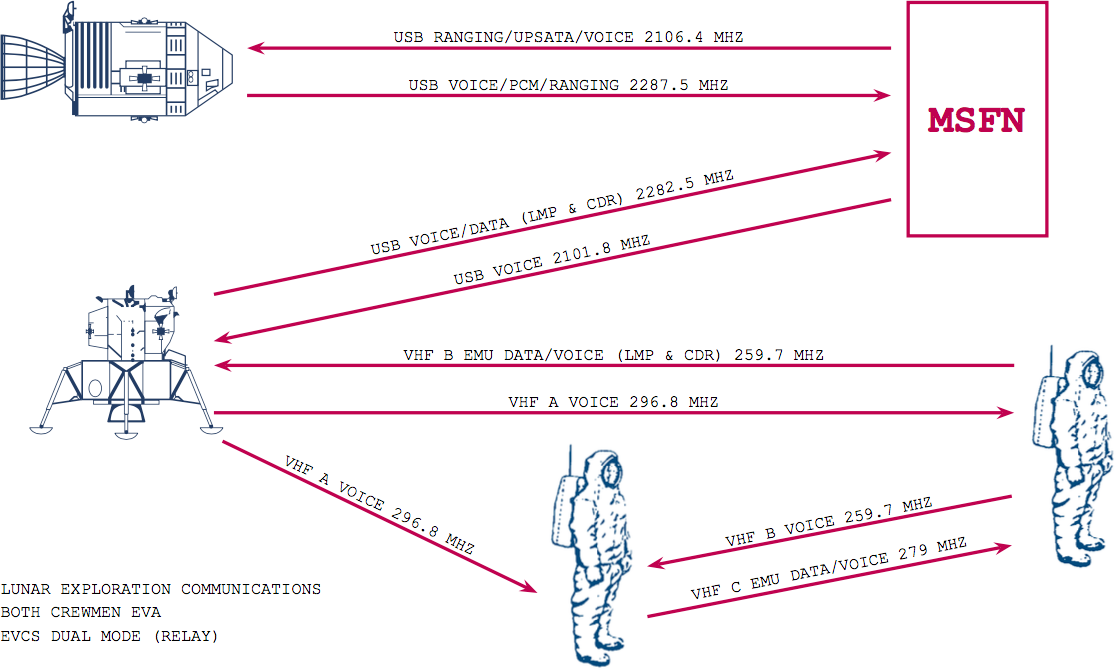
\includegraphics[width=\textwidth]{images/communication1.png}

% \subsection{No Car Camping}
% After checking in at the Greeter Station, you will be directed to unload your gear and then park your vehicle in the designated parking area, away from camping and event areas.  
% Only registered Art Cars, hybrid vehicles registered as generators (must be disguised and pimped out) or those needed by handicapped participants can stay with you at your campsite (must be covered up and decorated as well. They can't be driven during the event (with the exception of registered art cars)

% \subsection{Pets / Service Animals}
% \todo[inline]{BOD: please check; this is an abbreviated version that is more clear (to Raptor)}
% \begin{itemize}
% \item NO PETS ARE ALLOWED AT THIS EVENT
% \item Only working service animals are allowed on The Moon. Service animals are defined as dogs (or certain miniature horses) that are
%   \begin{itemize}
%   \item individually trained
%   \item identified as such to do work or perform tasks for people with disabilities.
%   \item Service animals must remain LEASHED and under control at ALL TIMES and will be asked to leave if the animal’s handler does not take effective action to control it.
%   \end{itemize}
% \item If you require a service animal to fully access the event, please inform us by no later than May 14, 2018 so that we can work with you to ensure comfort level for you and your service dog.
% \item No other animals may be brought or kept on the event premises. This includes
%   \begin{itemize}
%   \item Therapy animals
%   \item Emotional support animals
%   \item Personal pets
%   \end{itemize}
% \end{itemize}




% include vital info about participating in the burn, like guidelines, 10 principles and such
%
% This contains critical information regarding the burn, things like location,
% where the nearest hospital is located, definitions of terms, acronyms, the rules, 
% and information on any other burn-related resources.
%%
% This contains critical information regarding the burn, things like location,
% where the nearest hospital is located, definitions of terms, acronyms, the rules, 
% and information on any other burn-related resources.
%

\chapter{Astronaut Training}

\section*{Guidelines}
We have few rules and kindly ask you to follow them, for your safety and those around and with you.  Look at them as a compass to orient yourself by while drifting in the orbit of this event. 

\subsection*{Safety}
Safety is our number one concern and breaching perimeter is a \textbf{serious} offense we will handle swiftly. 

\subsubsection*{Fire Safety}
\begin{itemize}[noitemsep]
\item \textbf{\textcolor{red}{If you breach effigy or temple perimeter, you will be removed from the property immediately -- no questions asked!}} 
\item No open ground and / or unattended fires. They must be contained and off ground. Please bring a fire bowl for this purpose. If you see a fire that is unattended or out of control, contact a Ranger immediately.
\end{itemize}

\subsubsection*{River Safety}
\begin{itemize}[noitemsep]
  \item Children under 13 must wear a flotation device.
  \item Children under 13 must wear water shoes (water shoes are highly recommended for  \textbf{Anyone} for added safety and traction, especially if caught in a current).
  \item All minors must be accompanied by a parent or legal guardian when in the water.
  \item \textbf{Anyone caught committing the below two actions will be ejected from the burn immediately:}
  \begin{itemize}[noitemsep]
    \item No jumping or diving off the bank into the river.
    \item No swimming after dark.
  \end{itemize}
\end{itemize}

\begin{figure}[H]
\centering
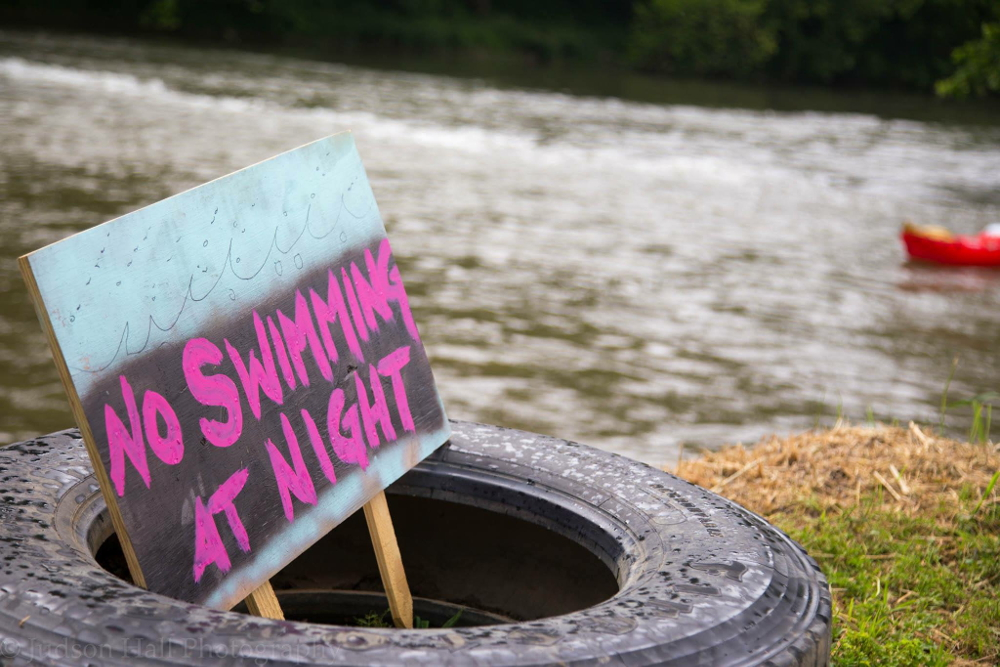
\includegraphics[width=.3\textwidth]{images/riversafety.jpeg}
\caption{No swimming at night. Image courtesy of Judson Hall Photography, 2016.}
\label{fig:2016riversafety}
\end{figure}

\clearpage
\subsection*{No Pets}
\label{sub:nopets}

Spirit Crossing has a \textbf{no pet} policy!

Should you need a service animal’s assistance to safely navigate our premises, please let us know at the gate.  A ``service animal'' is a dog (or other animal) individually trained to do work or perform certain tasks for a person with a disability.

Please be prepared to answer the following two questions so we may better determine at our discretion if your animal falls under the Service Animal Category, and in order for us to be in compliance with ADA regulations:

\begin{itemize}[noitemsep]
\item Is the service animal to the direct benefit of the disability?
\item What tasks and what work is the animal trained to perform in direct relation to the disability? 
\end{itemize}
 
If your animal falls under one of the following categories, you will not be able to bring it into the festival grounds.

Service Animals are \textbf{not}:
\begin{multicols}{2}
\begin{itemize}[noitemsep]
  \item emotional support animals
  \item therapeutic animals
  \item companion animals
  \item comfort animals
  \item service animals in training
\end{itemize}
\end{multicols}

For your convenience, Scooby Shack Kennel is 20 minutes from Sneedville and can be reached at 423-921-0611.

Thank you for your cooperation and understanding!

\begin{figure}[H]
\centering
	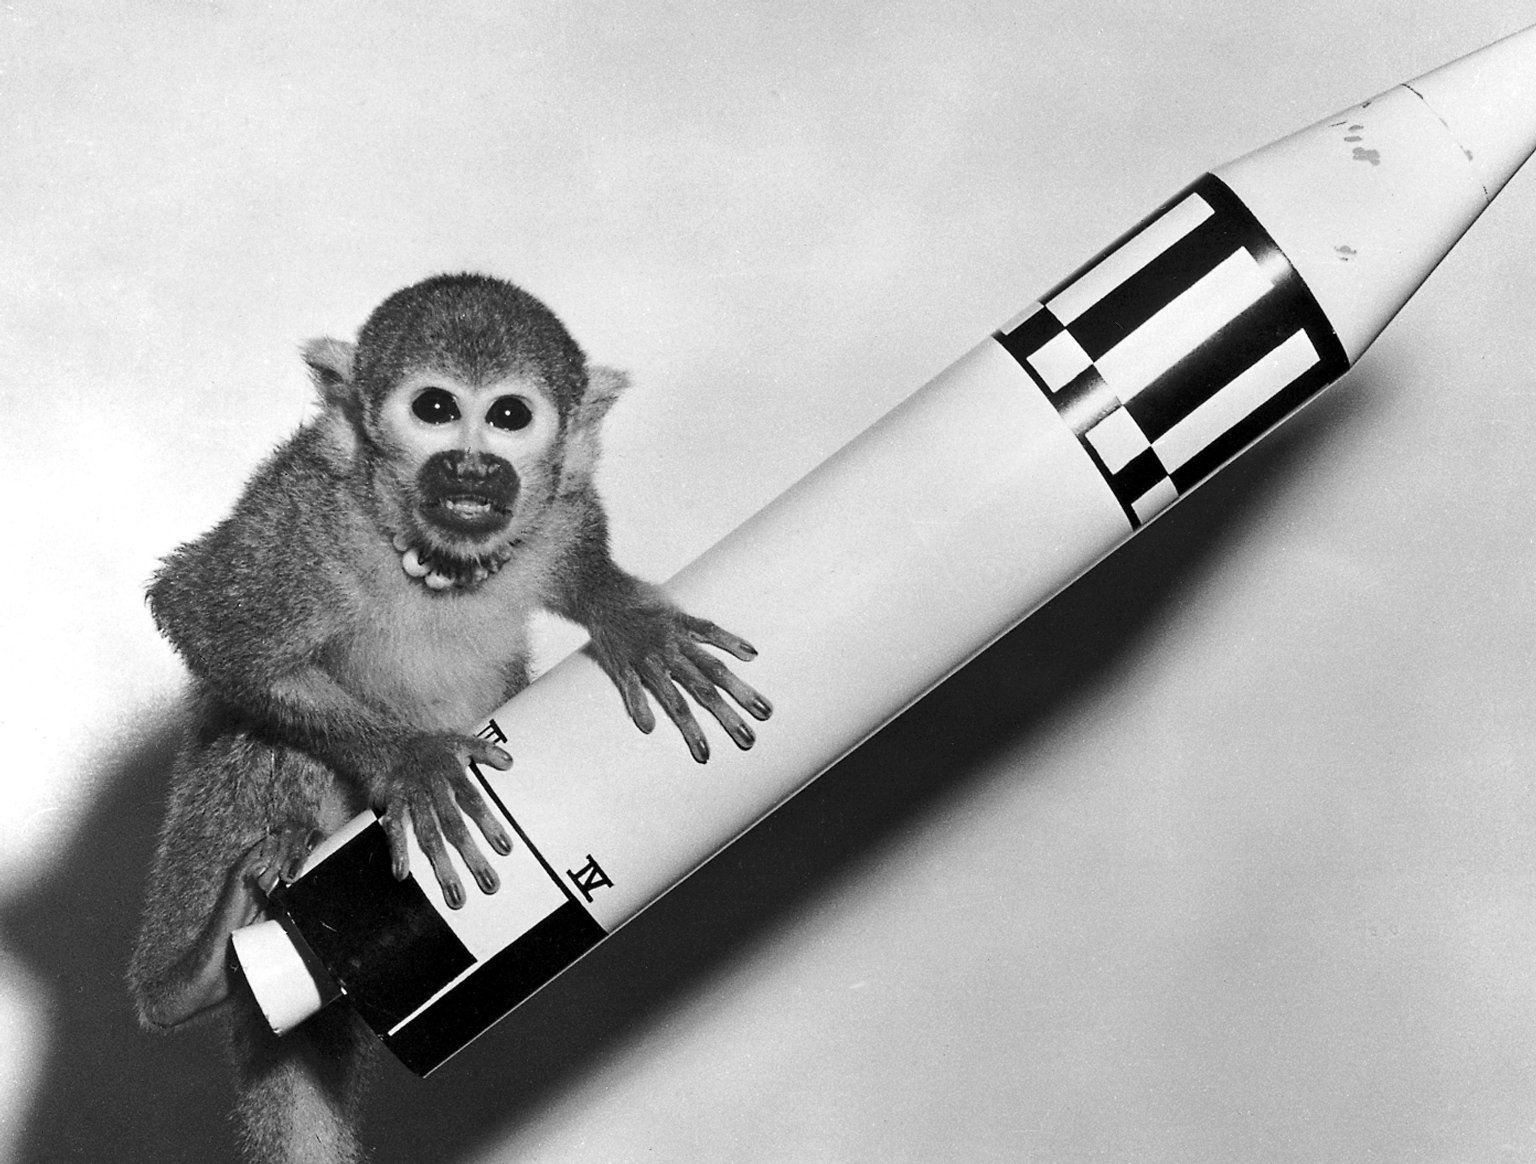
\includegraphics[width=.7\textwidth]{images/Baker}
    \caption{Miss Baker was a squirrel monkey who went into space and back in 1959. This is her on a model of Jupiter AM-18, the rocket that took her into space.}
    \label{image:missbaker}
\end{figure}

\clearpage
\subsection*{Respect the Laws of the Land}
Spirit Crossing, and Sneedville, are kind enough to be our home.  Here are some helpful tips on respect:
\begin{itemize}[noitemsep]
\item While the porch and patio may be used for specific team lead functions, the property owner’s house is off limits to participants.  Please be respectful of the land and grounds.
\item Although held on private property, TN Nudity Laws still apply.  To The Moon is an all ages event so please plan on wearing pasties, bikinis, loincloths, etc.
\item Please respect the land, the river, and the community.  Obey the speed limits and be courteous to those around you.
\item When in doubt, practice \textbf{consent}!
\item TTM  is an all ages event.  Those who are 21 or older will have a special wrist band indicating that they are able to legally consume alcohol. Please consume in moderation.
\end{itemize}
    
\begin{multicols}{2}

% \subsection*{Alcohol}
% \gls{ttm} is an all ages event.  Those who are 21 or older will have a special wrist band indicating that they are able to legally consume alcohol.

\subsection*{Camping}
You may not camp in your car. Please bring a tent or RV / trailer.
Cars may only be brought on site with approval.
% \bod[inline]{needs vetting}

\subsection*{Code of Conduct}
\Gls{ttm} now has a Code of Conduct. You can find it on page~\pageref{coc}.

\subsection*{Fireworks and Effects}
Fire effects with registered Theme Camps only, please.

\subsection*{\Gls{gifting}}\label{gifting}
This is a gifting community, providing refuge from everyday societal perils.  Once you're inside, no commercial activity takes place. Which is part of the charm, and the point :) 
Sometimes, there is a bit of a misconception of "Oh, so it's a barter system?" -- Actually, it's not. It's a "Gifting" Principle.
You gift without the expectation of a gift in return. 
You gift something to someone because at that moment, you feel the other person should have the very thing you'd like to give.

\subsection*{\Gls{graywater}}
There are no plans to dispose of gray water on site.  Each participant is responsible for \gls{pipo}.

% \subsection*{Nudity}
% TN Nudity Laws prohibit full or partial nudity on public property, and while we are on private property, the road cutting through Spirit Crossing is public, mostly accessed by residents, so very low traffic.

% We recommend you use discretion and wear pasties, paint, bikinis, etc.

\subsection*{Minors}
Minors must be accompanied by a parent or legal guardian. If they cause problems during the event which lead to possible safety issues or are a severe nuisance to others, we may ask you to remove the offending minor, possibly your entire camp. Minors are NOT allowed to use, play with, operate nor hold fire, fire props, fire effects and pyro, including poofers.  

%\subsection*{Public Health and Safety}

\subsection*{Recharging batteries for medical equipment}
Those with CPAPs and electronic scooters will have to make their own arrangements to recharge batteries.  \gls{ttm} does not provide battery recharging stations for medical equipment.

Some theme camps have generators, and may allow use of a spare generator plug for recharging medical equipment as a way of \gls{gifting}.  Home Depot and other companies also rent generators.  Moreover, there exist solar panels for recharging CPAP machines, though those can be prohibitively expensive.

% Not that this is now elsewhere in the document in the section on landing/exiting/etc.
% There is now also an explicit table that breaks down the gate hours by day.
% \subsection*{Re-Entry}
% Gate hours will be strictly adhered to unless prior arrangements have been made with event lead and / or property owner.
% Re-entry is prohibited unless
% \begin{itemize}[noitemsep]
% \item for medical reasons
% \item prior arrangements have been made
% % \item another invite is purchased 
% \end{itemize}
% Gate hours are 10 a.m. -- 10 p.m. Thursday and Friday, and 10 a.m. -- 6 p.m. Saturday.
% \bod[inline]{Are these hours correct? I got them off of a Dusty comment on Facebook.}

% \subsection*{Respect}
% Please respect the land, obey the speed limits, and be courteous to those around you.



\columnbreak
\subsection*{Photography}
Please respect the right of others who may not wish to be photographed. Ask \textbf{permission}! If you see someone with a \textcolor{blue}{blue} wristband, that is a \textbf{no photo} policy indicator. 
Do not take pictures or video of participants wearing them! 

% \subsection*{Property Owner's House}
% \todo[inline]{Home Base is not mentioned in the glossary. Is this the correct name?  And aren't the greeters near the site entrance?}
% While the porch and patio are used for \gls{greeter} Station and Home Base, the house is off limits to participants.  Please be respectful of the land and grounds. 

\subsection*{Sound}
To make this event enjoyable for all, amplified sound is limited to 300 Watts producing 90 db at 20 feet. All amplified sound is to be reduced after 4\am nightly to allow room for acoustic and ambient sound and to limit the possibility of neighboring sound complaints. 

\subsection*{Wristbands}
\label{sub:wristbands}
% \bod[inline]{needs vetting -- is the gate the correct location?}
You will receive a wristband when you arrive at the \gls{gate}.  Different colored wristbands will identify you as being over 21, under 18, etc.  Wristband colors also indicate if you don't want your photo taken.  

You must keep your wristband on at all times.  See the \gls{gate} if you need to replace your wristband.

\subsection*{Vending}
No vending, selling, or promoting is allowed at the event.
\end{multicols}

% \begin{tabular}{|p{6cm}|p{6cm}|} \hline
% \textbf{Do} & \textbf{Don't} \\ \hline \hline
% Follow safety protocols  & Breach effigy or temple perimeter               \\ \hline
% Camp in a tent or RV &  Camp in your car              \\ \hline
% Limit amplified sound to 90dB at 20 ft  & Bring your car on site+               \\ \hline
% Reduce amplified sound after 4 a.m. & Leave minors unattended               \\ \hline
% Obey TN nudity laws (cover up) & Sell, vend, or promote               \\ \hline
% Stay out of the property owner's house  & Leave fires unattended               \\ \hline
% Use fire bowls  & Start open ground fires               \\ \hline
% Respect land and neighbors  & Put anything but 1-ply toilet paper and human waste in portapotties               \\ \hline
% Ask permission before taking photos  & Take pictures of participants with green wristbands               \\ \hline
% Ask for consent  &   \\ \hline             
% \end{tabular}
% \vspace{2em}



\section*{Community Standards}

\subsection*{The Ten Principles}\label{tenprinciples}
Table \ref{tbl:tenprincples} enumerates the 10 Principles of \gls{ttm}.
Funny thing about those: they are not meant to be chosen at random to suit ones need, mood or agenda, but according to our interpretation were created to work together as a whole.  
Meaning your right to radically and freely express yourself ends when your expression infringes upon another participant to do the same. 

In other words, they're not a "Getting out of jail free" card, nor a permission slip to be a dick. So don't be a dick, hiding behind one or two principles. 

\begin{center}
	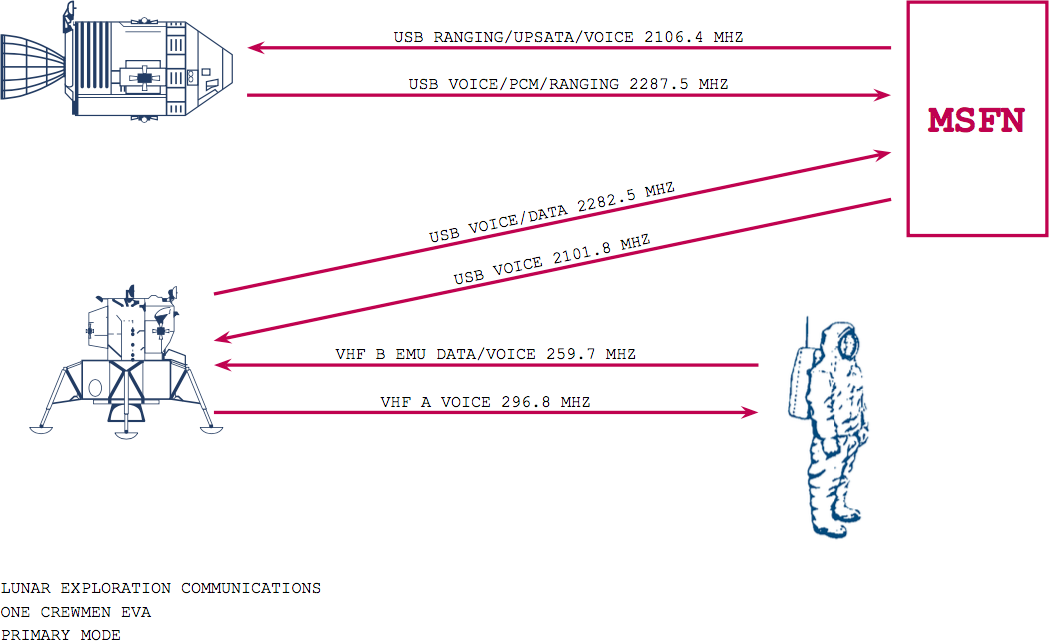
\includegraphics[width=.7\textwidth]{images/communication2}
\end{center}

\vspace*{\fill}
\begin{table}[h!]
\footnotesize
\centering
\caption[The 10 Principles]{The 10 Principles}
\label{tbl:tenprincples}
\begin{tabular}{@{}llp{4.3in}@{}}
\toprule
\textbf{No.} & \textbf{Principle}               & \textbf{Description}                                 \\ \midrule
1   & Radical Inclusion       & Everyone is welcome, all types, all kinds, friends, strangers, and in between.         \\[1em]
2   & Gifting                 & Gifts are unconditional offerings, whether material, service oriented, or even less tangible. Gifting does not ask for a return or an exchange for something else.        \\[1em]
3   & Decommodification       & Hand in hand with gifting, burns are environments with no commercial transactions or advertising. Nothing is for sale - we participate rather than consume.        \\[1em]
4   & Radical Self-Reliance   & You are responsible for you. Bring everything with you that you need. Burns are an opportunity for you to enjoy relying on yourself.          \\[1em]
5   & Radical Self-Expression & What are your gifts, talents, and joys? Only you can determine the form of your expression.         \\[1em]
6   & Communal Effort         & Cooperation and collaboration are cornerstones of the burn experience. We cooperate to build social networks, group spaces, and elaborate art, and we work together to support our creations.         \\[1em]
7   & Civic Responsibility    & Civic responsibility involves the agreements that provide for the public welfare and serve to keep society civil. Event organizers take responsibility for communicating these agreements to participants and conducting events in accordance with applicable laws.         \\[1em]
8   & Leaving No Trace        & In an effort to respect the environments where we hold our burns, we commit to leaving no trace of our events after we leave. This means everything that you bring with you goes home with you. Everyone cleans up after themselves, and whenever possible, we leave our hosting places better than we found them.            \\[1em]
9   & Participation           & The radical participation ethic means you are the event. Everyone works; everyone plays. No one is a spectator or consumer.        \\[1em]
10  & Immediacy               & From the Burning Man website : "Immediate experience is, in many ways, the most important touchstone of value in our culture. We seek to overcome barriers that stand between us and a recognition of our inner selves, the reality of those around us, participation in society, and contact with a natural world exceeding human powers. No idea can substitute for this experience."             \\ \bottomrule
\end{tabular}
\end{table}
\vspace*{\fill}


\clearpage
\subsection*{The 11th Principle -- Consent}

\gls{ttm} has adopted the 11th Principle, Consent\footnote{\url{http://www.11thprincipleconsent.org/2015/10/20/what-do-you-consent-to/}}.

\begin{labeling}{Photography:}
	\item[Touch:] Just because you hugged someone yesterday doesn't mean you can surprise them with a hug today. ``Surprise contact'' isn't always wanted, even if it's affectionate.
	\item[Kink:] Consent for one thing isn't consent for another. If I said you can spank me, that doesn't give you permission to grope me.
	\item[Sex:] Consent can be revoked once it's been given.
	\item[Gifts:] Disclose what is in your gifts, even if it's just essential oils. Some people have sensitivities.
	\item[Foods:] Disclose the ingredients, one person's innocuous ingredient can be someone else's allergy.
	\item[Photography:] Ask before taking pictures. Remember consent to take a picture is NOT consent to post it on your blog.
\end{labeling}


\section*{Code of Conduct}\label{coc}
TouchBass LLC / To The Moon Code are introducing a new Code of Conduct for 2018 and beyond.
If you are unable to agree to these terms and our policies, we’ll gladly issue a refund for your ticket.
Please contact us at connect@tothemoonburn.com. 

% \subsection*{The Moon Code Of Conduct}

\begin{multicols}{2}
To The Moon, produced by TouchBass LLC, relies on attendees and volunteers to create and maintain a space that is welcoming for all ticketed participants. We don’t discriminate on gender, sexual orientation, disability, ethnicity, socioeconomic status, age, or religion and we abide by the Burning Man 10 Principles.

Participation in this event is open to all ticketed attendees, but is a privilege nonetheless. Attending privileges of To The Moon and related events sponsored by TouchBass LLC will be revoked if a participant fails to respect other attendees or behaves in a way that endangers themselves, the event, or the broader community as a whole.
Damaging behavior is not limited to violence or consent violations, but rather includes ALL behavior detrimental to The Moon as a whole, the burn itself, affiliated events, TouchBass LLC, its BOD, Team Leads, and volunteers and other participants by means of any actions in direct contradiction to and out of alignment with our mission:

\emph{“To The Moon exists solely to create a platform allowing its participants to unfold their creative wings and embrace and nurture a community striving to share their passions, unique gifts and talents and come together in celebration to do just that.”}

We want to impose upon your freedoms within our chosen community as little as possible, but need to protect our members and event at the same time.
The following are our policies designed to do just that.
If you experienced anything in violation of these guidelines, please fill out our incident report form to help us investigate.

Please note: 3rd Party Incident Reports are not accepted. The report has to be submitted by the person directly involved in / with the incident. If you feel the need to report something as a 3rd Party, please email us at connect@tothemoonburn.com.

\subsection*{Expected behavior includes, but is not limited to}

% \begin{itemize}[noitemsep]
	\subsubsection*{Consent}
    \begin{itemize}[noitemsep]
    	\item Obtaining someone’s consent in a sexual context is absolutely mandatory
        \item Obtaining consent for video or photography of a participant, or in any other way which potentially affects the experience of another person on The Moon is mandatory
	\end{itemize}
        
    \subsubsection*{Non Consensual}
    \begin{itemize}[noitemsep]
        \item Be considerate and respectful of fellow participants and the community around the event.
        \item Refrain from non-consensual demeaning, discriminatory, or harassing behavior.
        \item Be mindful of your surroundings and of your fellow participants’ safety.
	\end{itemize}
% \end{itemize}

\subsection*{Unacceptable behavior includes but is not limited to}
\begin{itemize}[noitemsep]
    \item Predatory behavior, defined as any unwanted and non-consensual form of the following
    \begin{itemize}[noitemsep]
        \item Non-consensual physical contact, including unwelcome sexual interaction
        \item Intimidation, harassment, stalking
        \item Verbal or physical abuse
        \item Spousal abuse
        \item Violence against other participants or their property.
	\end{itemize}
         
    \item Abuse or neglect of To The Moon or land owner’s property, physical or otherwise, such as vandalism, theft of event property
     
    \item Sabotaging To The Moon, its Event Leads and other TouchBass LLC sponsored events, and the BOD by (including but not limited to)
    \begin{itemize}[noitemsep]
        \item Willfully perpetuating false information about TouchBass LLC’s operating procedure
        \item Intentionally damaging relationships fostered by To The Moon for future events by exhibiting aggressive or manipulative behaviors toward hosts and attendees of Touch Bass LLC events
        \item Deliberately harassing BOD members, Team Leads, volunteers or participants for the sole purpose of undermining TouchBass LLC Leadership, its BOD,  operating procedure, events and mission.  
	\end{itemize}

	\item Disrespecting the local community around the event by
    \begin{itemize}[noitemsep]
        \item Dumping trash in local dumpsters
        \item Trespassing
        \item Repeated violations of the event’s sound ordinance
    \end{itemize}

	\item Disregard for one’s own safety (including intentional self harm or intention of) or well-being to such an extent it demands the intervention of other participants, community members, Team and / or Event Leads. volunteers or outside agencies, such as intervention by local law enforcement or fire department staff.
    
	\item Repeated or egregious violations of any and all policies put in effect by event organizers.
    
    \item Defiance against Rangers or other Safety Team Leads, Event Leads and land owner handling a potentially dangerous or life threatening situation.
    
    \item Breaching Perimeter at any effigy / temple burn
\end{itemize}

\subsection*{Consequences of unacceptable behavior}
Unacceptable behavior will not be tolerated. This includes additional forms of said behavior at the burn as well as pre- or post-burn events and via all forms of communication across all platforms.

\textbf{Anyone asked to stop unacceptable behavior is expected to comply immediately.}

Participants who engage in unacceptable behaviors will be subject to event organizers action deemed appropriate to ensure the safety of the event, its affiliate events and affiliate relationships and its participants.
This action may include expulsion from the event without refund, revoking tickets, removing a volunteer from their shift, and temporary or permanent bans from TouchBass LLC events.

If a participant’s behavior does not comply with this code of conduct, does not align with our mission, or puts the future of TouchBass events at risk, (i.e. our burn, Town Halls, Fundraisers) a suspension for the present or following years may be imposed.
Suspensions may not be permanent, and appeals may be submitted in writing in cases where conflict resolution is demonstrated by the offending party. The appeal’s timeline is determined by TouchBass LLc and will be resolved between members of the Board and the suspended party.

TouchBass LLC or individuals may pursue potential legal action.
\end{multicols}

\vspace{2.75cm}

\begin{figure}[!h]
\centering
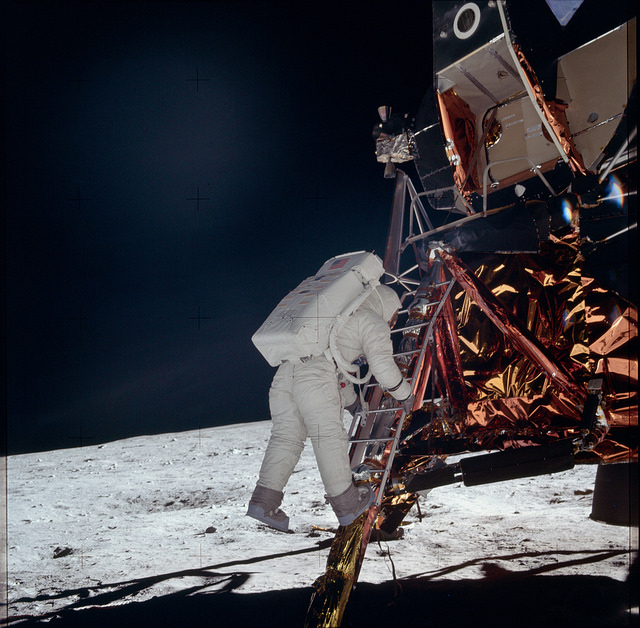
\includegraphics[width=.9\textwidth]{images/arrival.jpg}
% \caption{Astronaut climbing out of the }
\label{image:firststep}
\end{figure}



% Information about the teams, which will be a natural segue to volunteering for some of them
%
% Descriptions of the various teams.  Volunteering section will refer to this.
%


\chapter{Crew Manifest}
\label{ch:teams}


These are all the teams that support \gls{ttm}.  You can contact these teams or the \gls{ttm} leadership by sending email to \url{connect@tothemoonburn.com}.  Each team also has its own contact email, which is given below.
% * <mcoletti@gmail.com> 2018-05-05T21:21:35.396Z:
% 
% > These are all the teams that support the \gls{ttm}.
% Expand on this.
% 
% ^.

% \begin{multicols}{2}

\vbox{
\subsection*{Board of Directors}
The Board of Directors oversees \gls{ttm} at large.
\begin{description}[leftmargin=6em,noitemsep,style=nextline]
    \item[Leads] Gabi ``Nectarine'' Stewart, Andrea Kerns, Ashley ``Bones'' Abbott, Brad ``Bradass'' Tomlinson, Tonya ``Dusty Lashes'' Weisenseel
   \item[Contact:] \url{connect@tothemoonburn.com}
\end{description}
}

\vbox{
\subsection*{Flight Directors / Event Leads}
The \gls{eventleads} are the acting managers during the event itself.  Through close communication with each Team Lead, they effectively ensure  that all on-site operations run smoothly.  And they drive golf carts.

\begin{description}[leftmargin=6em,noitemsep,style=nextline]
   \item[Leads:] Vicki ``Critter'' Coleman, Ben ``Cheesepants'' Bjostad, Ann ``Mango'' Gerns
   \item[Contact:] \url{connect@tothemoonburn.com}
\end{description}
}

\subsection*{ART Team}
The Art Team stays connected with artists from initial inquiry about Art Registration and / or Art Grant Application, communicates with safety teams and BOD about amounts granted, fire and other safety concerns regarding interactive art and about feasibility and scope of art projects. Art Team also works closely with placement to ensure the best spot for any art projects. 

\begin{description}[leftmargin=6em,noitemsep,style=nextline]
   \item[Lead:] Carrie ``Minx'' Elliot
   \item[Co-leads:] Louise Marie ``Vortex'' Fry, Karine Monica Martelly
   \item[Contact:] \url{artgrants@tothemoonburn.com}
\end{description}

\vbox{
\subsection*{Conclave / Fire Prop Safety}
This team is responsible for the conclave fire spinning event that occurs just before the \gls{effigy} and \gls{temple} burn.

\begin{description}[leftmargin=6em,noitemsep,style=nextline]
   \item[Lead:] Elaine Pastor
   \item[Co-leads:] Alicia ``Alley Hoops'' Westbrook
   \item[Contact:] \url{conclave@tothemoonburn.com}
\end{description}
}

\subsection*{DPW}
The \gls{dpw} team is responsible for handling the event's logistics, electrical power management, and infrastructure.

% \gls{dpw} is looking for \glspl{shiftlead} to cover all of the listed shifts.  Please contact \gls{dpw}  if you are interested in becoming a \gls{shiftlead}.

% % I used the addmargin to give this description list a little nudge to 
% % prevent confusion for the description lists used for the leads/co-leads
% \begin{addmargin}[.3cm]{0cm}
% \begin{description}[noitemsep]
% % 	\item[DPW:] The team here to take care of the infrastructure, and help keep the wheels on the bus.
% 	\item[Doozers:] "Do" The Things: Can get things done: lift, tote, dig
% 	\item[Dispatch:] Organized Soul, Radio trained, likes clipboards - must be approved by \gls{dpw} lead
% 	\item[Burn Down:] Preps structure for burn down.
% \end{description}
% \end{addmargin}

\Gls{dpw} meets at \gls{groundcontrol}.

\begin{description}[leftmargin=6em,noitemsep,style=nextline]
   \item[Lead:] Ian ``Little Buddy'' Brinn, Jack Holloway
   \item[Co-leads:] Daniel Goodridge, Sara ``Beastmode'' Vaughn Wright
   \item[Contact:] \url{DPW@tothemoonburn.com}
\end{description}

\subsection*{Effigy}
This team is responsible for the construction of the main effigy burned on Saturday night.

\begin{description}[leftmargin=6em,noitemsep,style=nextline]
   \item[Lead:] Brad ``Bradass'' Tomlinson
   \item[Co-leads:] Karine Monica Martelly
   \item[Contact:] \url{effigy@tothemoonburn.com}
\end{description}

\subsection*{Fire Safety}
This teams helps provide a safe environment for fire art, the \gls{effigy}, and the \gls{temple}. They patrol the burn to help make sure that fire art and fire performance are safely done.

% \begin{addmargin}[.3cm]{0cm}
% \begin{description}[noitemsep]
% 	\item[Dirt Patrol:] Looks for fires out of place and ensures that fire spinners are spinning safely.
% \end{description}
% \end{addmargin}

% This year we are combining Fire Safety with \gls{rangers}. If you have experience and would like to be a part of the Fire Safety Team, we need you. Please contact the Fire Safety Lead, Critter, directly to sign-up for these shifts. We are directing everyone to \gls{rangers} shifts. We will have onsite training for Fire Safety and Rangering!

\begin{description}[leftmargin=6em,noitemsep,style=nextline]
   \item[Lead:]	Dave ``Phyrebolt'' Peters
   \item[Contact:] \url{firesafety@tothemoonburn.com}
\end{description}


\subsection*{Gate}
The \gls{gate} team is the first to welcome participants home, takes invites, id's, signed waivers, and records emergency contact info.

This team meets at the \gls{launchpad}.

\begin{description}[leftmargin=6em,noitemsep,style=nextline]
   \item[Lead:] Amy Nichols
   \item[Co-leads:] Reida Gillespie, Sarah Hurst
   \item[Contact:] \url{gate@tothemoonburn.com}
\end{description}


\subsection*{Greeters}
% These are the kind and gentle folks that welcome you home.  They will check your tickets, put on your wristbands, and will help orient you on where to go and what to do at \gls{ttm}.  They also make sure that all arriving crew members are aware of and will adhere to the \gls{tenprinciples} and the \gls{eleventhprinciple}.

\paragraph{Who We Are}
We are the brightly shining faces of To The Moon.  We are the ones that will help you blast off into a world of beauty you've never known.

\paragraph{What We Do}

As Greeters, we are the first group to welcome astronauts to the Launch Pad, and we absolutely love doing it!  We, along with Gate, make the first impression on this voyage.  We help set expectations and get to communicate with the flight crew for the very first time. 

Our job is to educate ourselves deeply on the meaning of the \gls{tenprinciples} so that we can impart that knowledge onto our participants.  We're also well versed in the \gls{eleventhprinciple} and are happy to discuss!  We are here to clarify any questions you have regarding general operating procedures on the Moon. 

% We are passionate about the beautiful land that is Spirit Crossing, and have educated ourselves deeply on the history of the land and special facts that are critical to understand in order to give back to nature the way she gives to us. 

% Looking for some sweet \gls{swag}? Look no further than the \gls{greeter} station!  Want a good spanking?  Hey, if you say it's ok, then we're ok with it!  Have questions about where to go to sign up to volunteer? We got it!  Interested in picking up a ``No Photos'' wristband? That's covered, too!  Want to know which camps are kid-friendly?  Done and done!

% Greeters are all about having FUN!  Our goal is to get you excited about coming home!  We want everyone to be safe and knowledgeable and have a hell of a time doing it!   

\paragraph{What We Need}

We are looking for outgoing, space-age, creative people to join our band of misfits.  If you are dedicated, patient, have great communication skills, and are ready to take on the truly awesome role of creating out-of-this-world merriment and moon-like magic, then volunteer with us. 

See you on the Moon!!!!

The \glspl{greeter} meet at the \gls{launchpad}.

\begin{description}[leftmargin=6em,noitemsep,style=nextline]
   \item[Lead:] Kris ``funsized'' Long
   \item[Co-leads:] Andi ``Glytch'' Long, Corey Anne
   \item[Contact:] \url{greeters@tothemoonburn.com}
\end{description}

% These are the kind and gentle folks that welcome you home.  They will check your tickets, put on your wristbands, and will help orient you on where to go and what to do at \gls{ttm}.  They also make sure that all arriving crew members are aware of and will adhere to the \gls{tenprinciples} and the \gls{eleventhprinciple}.

\vbox{
\subsection*{Moon Ice}

These volunteers will oversee the moon ice sales each day from 12-3pm

\begin{description}[leftmargin=6em,noitemsep,style=nextline]
   \item[Lead:] $\emptyset$
   \item[Co-leads:] $\emptyset$
   \item[Contact:] \url{volunteer@tothemoonburn.com}
\end{description}
}

\subsection*{\Gls{lamplighters}}
These participants gather before dusk to ceremonially light our moonbase with lanterns, and then gathers them each morning.   
% The \gls{lamplighters} is a burner tradition that started in 1993.  The \gls{lamplighters} are a somber procession starts at twilight each night to kindle torches to help light our way through the night.

Meets at the \gls{cockpit}.

\begin{description}[leftmargin=6em,noitemsep,style=nextline]
   \item[Lead:] Johnny ``Twaffle'' Benton
   \item[Co-leads:] Melody Shah,  Bryan Shah
   \item[Contact:] \url{lamplighters@tothemoonburn.com}
\end{description}


\subsection*{Leave No Trace}
These crew members are responsible for ensuring that the grounds are as we found them --- free of any artifacts of our presence, such as bottle caps, empty bottles, forgotten items, and any other \gls{moop}.

\begin{description}[leftmargin=6em,noitemsep,style=nextline]
   \item[Lead:] Henry ``Jawk'' McElreath
   \item[Co-leads:] Mandy Kees
   \item[Contact:] \url{LNT@tothemoonburn.com}
\end{description}


\subsection*{Parking / L.O.V.E. / GTFIO}
These crew members are responsible for the efficient and safe landing of all vehicles, and for their orderly and speedy departure.  \Gls{gtfio} is responsible for overall landing and takeoff of vehicles; \gls{love} helps extract vehicles mired on the lunar surface.

\begin{description}[leftmargin=6em,noitemsep,style=nextline]
   \item[Lead:] Kent ``Pop'' Davis
   \item[Co-leads:] Brandon ``Naked Light''
   \item[Contact:] \url{parking@tothemoonburn.com}
\end{description}

% These crew members are responsible for the efficient and safe landing of all vehicles, and for their orderly and speedy departure.  \Gls{gtfio} is responsible for overall landing and takeoff of vehicles; \gls{love} helps extract vehicles mired on the lunar surface.

\subsection*{Perimeter}
These participants meet up before burn time and establish a burn perimeter to aid in the safety of participants during the \gls{effigy} and \gls{temple} burns.

Perimeter signup only includes \textbf{outer} perimeter shifts (no experience needed other than a mandatory training session (see times above). If you are experienced with perimeter and fire safety and want a shift doing \textbf{inner} perimeter, please email the perimeter lead directly and they will vet you for that.

Meets on the Burn Field

\begin{description}[leftmargin=6em,noitemsep,style=nextline]
   \item[Lead:] Vicki ``Critter'' Coleman and Ben ``Cheesepants'' Bj{\o}st{\aa}d
   \item[Co-leads:] $\emptyset$
   \item[Contact:] \url{perimeter@tothemoonburn.com}
\end{description}


\subsection*{Placement}
This team ensures proper placement of all Theme Camps to avoid sound bleed and bad neighborly relations, creates open camping areas and basically creates the layout of our entire event. Placement works side by side with TCOs and BOD and the end result is our beautiful placement map which you'll find in this survival guide, at the gate and Cockpit. 
\begin{description}[leftmargin=6em,noitemsep,style=nextline]
   \item[Lead:] Caleb Ditchfield
   \item[Co-leads:] Josh Blackwood
   \item[Contact:] \url{placement@tothemoonburn.com}
\end{description}

% This team assigns locations for theme camps and other temporary emplacements.

\newpage
\subsection*{Rangers}
% \Gls{rangers} are responsible for keeping the peace.
Rangers are the non-confrontational mediators of community and public safety and providers of information. While on shifts they will carry radios. They are super cool. They stroll the burn and are often the first point of contact should you need assistance.

% I used the addmargin to give this description list a little nudge to 
% prevent confusion for the description lists used for the leads/co-leads
\begin{addmargin}[.3cm]{0cm}
\begin{description}[noitemsep]
	\item[Khaki:] Experienced Ranger running shift, also serves as khaki (dispatch/coordination). Email the Ranger Lead, Runs with Scissors, to sign-up for these shifts.
	\item[Dirt Patrol:] Experienced Ranger, paired with an alpha. For this first burn, both rangers may be inexperienced and if so, will receive on-shift mentoring from lead.
	\item[Alpha:] Inexperienced ranger, paired with a "dirt" ranger. If no dirt ranger available, that's ok. New burn. We will mentor during shift.
\end{description}
\end{addmargin}

Meets at \gls{missioncontrol}.
\begin{description}[leftmargin=6em,noitemsep,style=nextline]
   \item[Lead:] Don ``Runs With Scissors'' Coleman
   \item[Co-leads:] Alan ``Weatherman'' Huskey, Robert Blew
   \item[Contact:] \url{rangers@tothemoonburn.com}
\end{description}


\subsection*{Survival Guide}
\label{sec:survivalguide}
The \gls{survivalguide} team is responsible for the creation, printing, and distribution of the \gls{preflightmanual} and \gls{survivalguide}. We hope you enjoy this guide and find it helpful!

\begin{description}[leftmargin=6em,noitemsep,style=nextline]
   \item[Lead:] Andy ``Raptor'' Berres
   \item[Co-leads:] Mark ``Piprrr'' Coletti
   \item[Contact:] \url{survivalguide@tothemoonburn.com}
\end{description}


\subsection*{Tbase / Sanctuary}

\Gls{tbass} provides a calm, safe space for burners who need a chance to process and integrate their experiences at and responses to the burn. We provide a supportive environment for anyone who needs reassurance, assistance, or just some peace and quiet to work through a current experience or their response to a previous experience. A burn provides a multitude of stimuli, and \gls{tbass}  offers a chance to step back, ground oneself, and experience the transformative process that being home can bring.

Volunteers should be prepared to be sober and unaltered for the duration of a 4-hour shift and able to remain calm when dealing with participants who are distressed, emotional, or experiencing an altered perception of the world around them. 

% Volunteers should be prepared to be sober and unaltered for the duration of a 4-hour shift and able to remain calm when dealing with participants who are distressed, emotional, or experiencing an altered perception of the world around them. Anyone who has previously done Tranquility Base training for Alchemy or Euphoria, Sanctuary training for Ignite!, Transformus, or Flipside, or Zendo Project training for Burning Man can sign up for volunteer shifts now and only needs to attend a brief refresher session and an overview of To The Moon radio protocols (if you have done training for harm reduction/safe space teams at other burns, please contact Mango, the Tranquility Base Team Lead, to discuss your background). If you have not done training, please plan to attend one of the on-site training sessions on Thursday or Friday evening, and you will be able to sign up for volunteer shifts later in the burn at the end of the training or you may sign up for shifts now as long as you attend a training before your shift is scheduled.

Please plan to attend one of the on-site training sessions or refresher sessions.

This team meets at \gls{tbass}, of course.

\begin{description}[leftmargin=6em,noitemsep,style=nextline]
   \item[Lead:] Jo Herrera
   \item[Co-leads:] Stan ``MK'' Davis, Kristin Pereira
   \item[Contact:] \url{tbase@tothemoonburn.com}
\end{description}


\subsection*{Temple}
This crew assembles and deploys the \gls{temple} to be burned on the last night of \gls{ttm}.

Please note that a few hands are needed to help clean up on Monday after the Temple burn from the night before. Please be sure to pack up your camp before reporting for this shift as the burn will be ended and this shift requires ``late stay'' permission.

\begin{description}[leftmargin=6em,noitemsep,style=nextline]
   \item[Lead:] Sara
   \item[Co-leads:] $\emptyset$
   \item[Contact:] \url{temple@tothemoonburn.com}
\end{description}

% This crew assembles and deploys the \gls{temple} to be burned on the last night of \gls{ttm}.
% \columnbreak

\subsection*{\acrlong{vc}}
% \Gls{ttm} runs on volunteers, and this stalwart crew makes sure that all the teams have the necessary folks to work effectively.
These volunteers wrangle participants of the burn into needed volunteer positions to keep things running. \glspl{vc} help people check their scheduled shifts as well as sign up for shifts. If you know how sexy volunteering is and want to meet like minded folks, this is a good team for you! We keep volunteers informed of updates during the burn and help teams fulfill unforeseen volunteer needs as they could arise during the burn.

This is also a place for people to come get information about burn happenings, times, locations, and whereabouts to things such as: workshops, theme camps, and events. Sometimes we even help people find themselves!

This team meets at the \gls{cockpit}.

\begin{description}[leftmargin=6em,noitemsep,style=nextline]
   \item[Lead:] Julie Reach
   \item[Co-leads:] Shelli Renee
   \item[Contact:] \url{volunteer@tothemoonburn.com}
\end{description}

% how we can each contribute to the burn
%
% Here are the many ways folks can help out.
%
% TODO I know I'm missing lots.  :-\
%

\chapter{Volunteering}

No burn exists without volunteers and volunteers are our heroes! We have no hired help other than security and everything we do is done on a volunteer basis.  This goes for all the things before, during, and after the burn.  All the teams that you can volunteer for are described in the ``Crew Manifest'' section starting from page \pageref{ch:teams}.

There are two ways to volunteer:

\textbf{Before the event} you can sign up from the available volunteer activities by going to:

{\indent ~~~ \url{https://www.signupgenius.com/tabs/33773df01a4c3edc42-tothemoon} }

\textbf{During the event} you can go to the \gls{vc} folks at the \gls{cockpit} to sign up for an available volunteer slot.

\section*{EARLY ENTRY FOR VOLUNTEERS}

If a participant has a volunteer shift on Wednesday, they will be granted entry at noon on Wednesday. \footnote{This is mainly \gls{gate} but a few other teams have a few volunteer shift scheduled for Wednesday for set up.}  If a participant has a volunteer shift beginning before noon on Thursday they will be granted early entry on Wednesday after 3 pm.  This list will be given to \gls{gate} from \gls{vc} before \gls{gate} opens opens on Wednesday.

All participants must be off site by noon on Monday unless they have a shift on Monday after noon. In which case they will need to have permission from \gls{vc} or one of the \gls{eventleads} to stay on site for that shift, and should stop by the \gls{vc} tent on Monday before 10 am to get their approval. All late stay volunteer must also have their camp packed before their shift on Monday and be prepared to leave immediately following that last shift.\footnote{There are other early entries granted for \glspl{themecamp}, \gls{dpw}, \glspl{teamleads}, \gls{bod}, etc,,  but those lists will be given to \gls{gate} from appropriate lead for that team. This info is just for those volunteering first shifts on teams that start when gates open or before.}


\clearpage
\section*{Volunteer Training}

\subsection*{Conclave}
We ask that all fire spinners attend one of the the three fire safety meetings provided by Singe City and obtain a wristband. This will allow you to come spin in their fire circle each night in Headroom Village. 

Fire safety meeting will be at Singe City fire circle in Headroom Village:
Spinners in conclave must attend one of the training events listed below.
You will be given a fire safe wristband to spin fire during the burn. Conclave participants should meet at \gls{effigyburnfield} at 3:00\pm{} Saturday evening.

\begin{center}
\begin{tabular}{|c|c|c|}
\hline
\textbf{Day} & \textbf{Time} & \textbf{Place} \\ \hline
Thursday & 5\pm{} & Singe City fire circle in Headroom Village \\ \hline
Friday & 5\pm{} & Singe City fire circle in Headroom Village  \\ \hline
Saturday & 5\pm{} & Singe City fire circle in Headroom Village  \\ \hline
\end{tabular}
\end{center}

% \clearpage

\subsection*{Perimeter}
Outer Perimeter volunteers meet at the \gls{effigyburnfield} on before the burn at the times listed below for training/instructions. Friday and Sunday for the two temple burns, volunteers will stay at the \gls{effigyburnfield} until the burn. Saturday, the training is well before the burn. Volunteers will be given a break, and meet again at the specific time given at training.

If you are experienced with perimeter and fire safety and want a shift doing \textbf{inner} perimeter, please email the perimeter lead directly (\url{perimeter@tothemoonburn.com}) and they will vet you for that.

\begin{center}
\begin{tabular}{|c|c|c|}
\hline
\textbf{Day} & \textbf{Time} & \textbf{Place} \\ \hline
Friday & 8:15\pm{} & \gls{effigyburnfield} \\ \hline
Saturday & 4\pm{} & \gls{effigyburnfield} \\ \hline
Sunday & 6:30\pm{} & \gls{effigyburnfield} \\ \hline
\end{tabular}
\end{center}


\subsection*{Rangers and Fire Safety}

\begin{center}
\begin{tabular}{|c|c|c|}
\hline
\textbf{Day} & \textbf{Time} & \textbf{Place} \\ \hline
Thursday & 7\pm{} & \gls{moonrangerstation} \\ \hline
Friday & 1\pm{} & \gls{moonrangerstation} \\ \hline
Saturday & 1\pm{} & \gls{moonrangerstation} \\ \hline
\end{tabular}
\end{center}

\subsection*{River Safety}

Note that this safety training is open to everyone.  Anyone that wants to play in the river is strongly encouraged to attend.

\begin{center}
\begin{tabular}{|c|c|c|}
\hline
\textbf{Day} & \textbf{Time} & \textbf{Place} \\ \hline
Friday & 1:30\pm{} & Riverfront below \gls{dpw} \\ \hline
\end{tabular}
\end{center}

\vbox{
\subsection*{Tbase / Sanctuary}
You will also be able to sign up for volunteer shifts at the burn, at the end of the training, or you may sign up for shifts now as long as you attend a training before your shift is scheduled.

\begin{center}
\begin{tabular}{|c|c|c|}
\hline
\textbf{Day} & \textbf{Time} & \textbf{Place} \\ \hline
Thursday & 6\pm{} & \gls{tbass} \\ \hline
Friday & 7\pm{} & \gls{tbass} \\ \hline
\end{tabular}
\end{center}}

% \bod[inline]{add all volunteer training}
% \todo[inline]{Add information on how to volunteer before and during the event. Probably from https://www.tothemoonburn.com/volunteering}
\vfill
\begin{figure}[H]
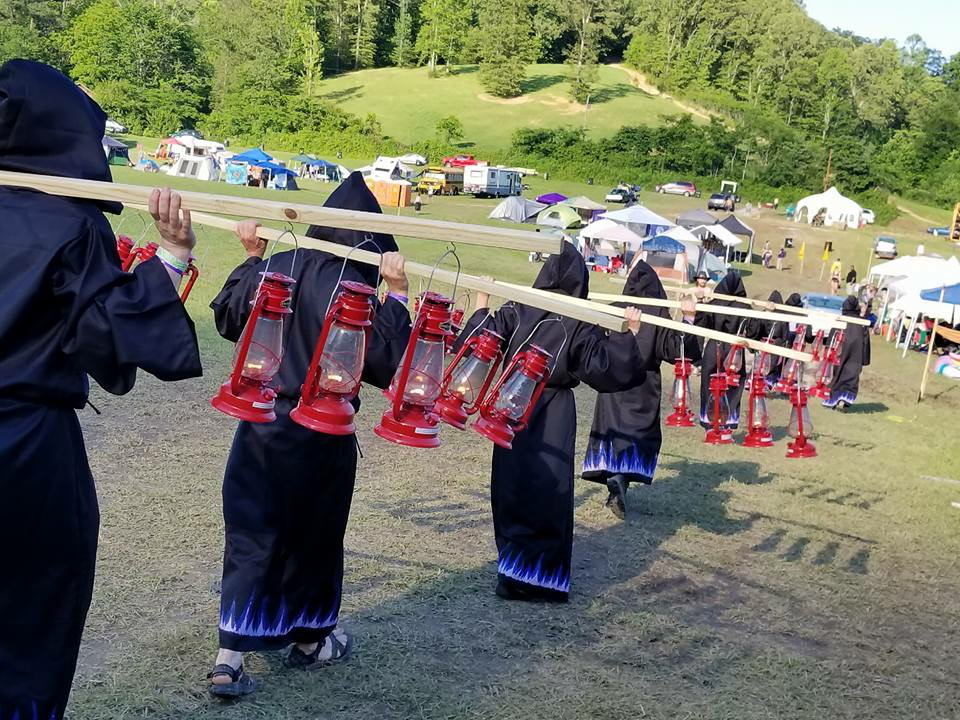
\includegraphics[width=\textwidth]{images/lamplighters.jpeg}
\caption{Lamplighters at work. Image courtesy of Johnny “Twaffle” Benton, 2017.}
\label{fig:lamplighters2017}
\end{figure}


% glossary
\appendix
% \appendixpage
\addappheadtotoc
% \addcontentsline{toc}{chapter}{Appendix}
\chapter{Terms and Definitions}

% Force printing of all glossary entries, even if not referenced.
\glsaddall

\begin{multicols}{2}
\printglossaries
\end{multicols}

\vspace*{\fill}
\begin{center}
	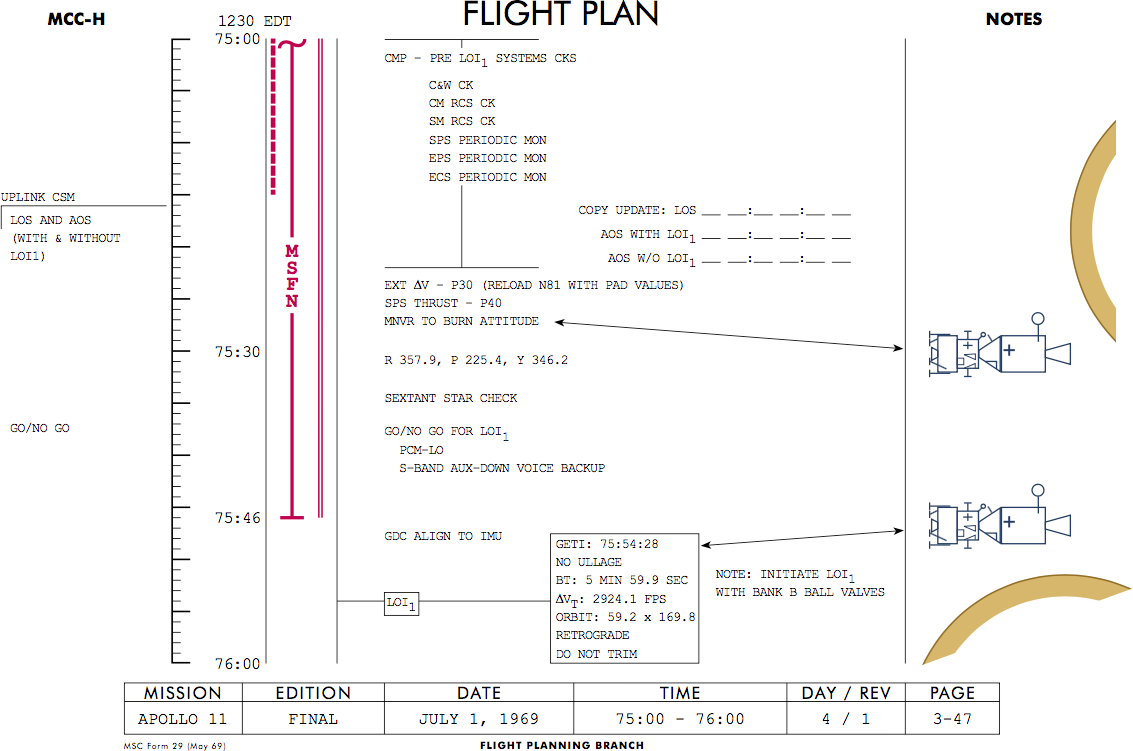
\includegraphics[width=.9\textwidth]{images/flightplan3}
\end{center}
\vspace*{\fill}

\clearpage

\chapter{Acknowledgements}
\section*{Image Credits}

\begin{multicols}{2}
\subsection*{Title Page} 
Andy ``Raptor'' Berres

\subsubsection*{Sources:}
\begin{itemize}[noitemsep]
  \item Galaxy texture: NASA Image Library \url{https://images.nasa.gov/}
  \item Astronaut and moon surface: Project Apollo Archive \url{https://www.flickr.com/photos/projectapolloarchive/}
  \item Alchemy Element Symbols: public domain
  \item Cat picture: Andy ``Raptor'' Berres
  \item Layout inspiration: Apollo Flight Manual \url{https://www.hq.nasa.gov/alsj/a11/a11fltpln_final_reformat.pdf}
\end{itemize}
\vfill\null

\subsection*{TTM 2018 Artwork}
Thomas O'Connor

\subsection*{Maps}
\begin{description}[leftmargin=6em,noitemsep,style=nextline]
	\item[Direction maps:] Andy ``Raptor'' Berres
	\item[Inside back cover map:] Mark ``Piprrr'' Coletti
\end{description}

\columnbreak



\subsection*{Photos}
\begin{itemize}[noitemsep]
\item Various Apollo Mission photos: Project Apollo Archive \url{https://www.flickr.com/photos/projectapolloarchive/}, NASA
  \item Mountain moon on page \pageref{image:mountainmoom}: \url{https://commons.wikimedia.org/wiki/File:Shenandoah_National_Park_SHEN4850.jpg}
  \item Buzz Aldrin on the Moon on page \pageref{image:buzzaldrin}: \url{https://commons.wikimedia.org/wiki/File:Aldrin_Apollo_11.jpg}
\item 2016 No Swimming at Night sign on page \pageref{fig:2016riversafety}, Judson Hall Photography
\item 2017 Lamplighters on page \pageref{fig:lamplighters2017}, Johnny ``Twaffle'' Benton
\item 2017 Light tunnel on page \pageref{image:tunnel}, Ashley ``Bones'' Maynard
\item 2017 Effigy burn on page \pageref{image:2017effigyburn}, Piprrr
\item Monkey Baker with a Model Jupiter Vehicle on page \pageref{image:missbaker}: \url{https://archive.org/details/MSFC-5909731}
\end{itemize}


\subsection*{Diagrams}
\begin{itemize}[noitemsep]
\item Various Apollo Mission diagrams: Apollo Flight Manual \url{https://www.hq.nasa.gov/alsj/a11/a11fltpln_final_reformat.pdf}
\end{itemize}

\subsection*{Swag}

\begin{description}[leftmargin=6em,noitemsep,style=nextline]
	\item[Design:] Andrea Kerns
  \item[Creation:] Dylan Talley
\end{description}

\end{multicols}

\clearpage
% We may want to expand this to include all volunteers/leads/co-leads.  Not only
% to acknowledge them ... BUT THIS MEANS A BIGGER HEART!  And we like biggger hearts!

% \topskip0pt
\vspace*{\fill}
\begin{center}
\Large
\textbf{Thank you!}
\end{center}

% \todo[inline]{add photo credits and other tips of the hat}
% We will be adding more and more to this list in the weeks leading up to the event.


\shapepar{\heartshape}
For providing valuable feedback and contributions, the Survival Guide team would like to thank Ben Secrest, Sharon Burdick, Dusty Lashes, Willow Gaia, Kris Long, Andi Glytch, Andrea Kerns, Aley Maurizio, Rebekah Lührs, Abigail Anniemal, Julie Reach,  Katie ``Creamy'' Miller, and Ben ``Cheese Pants'' Bj{\o}st{\aa}d. For their contributions, we would also like to thank all artists, theme camp organizers, and event organizers.  We would also like to thank the Hancock county sherrif's and fire departments for their support.

\bod[inline]{BOD/Teams: who else needs to be acknowledged?}
\vspace*{\fill}

% \chapter*{Notes}

\chapter{Site Map}

\section*{Theme Camp Map Index}
\subsection*{Alphabetical Order}
\begin{multicols}{2}
% \small
\begin{itemize}[itemsep=.0125mm,parsep=2pt]
   \item[\textbf{ 44 }] 3rd Aid
   \item[\textbf{ 4 }] Acrodesiac Lunartics
   \item[\textbf{ 33 }] Alcoholic Alliterators
   \item[\textbf{ 10 }] As Above So Below- Dreams of Flying
   \item[\textbf{ 7 }] Barefoot Barbaloots
   \item[\textbf{ 12 }] Black Lodge
   \item[\textbf{ 39 }] Brownie Brothel
   \item[\textbf{ 13 }] Burning Yacht Club
   \item[\textbf{ 6 }] Camp Do it Less Shitty
   \item[\textbf{ 48 }] Camp Hell Yeah!
   \item[\textbf{ 46 }] Camp PFA
   \item[\textbf{ 27 }] Camp Quasar
   \item[\textbf{ 35 }] Clean Hippies Taste Better
   \item[\textbf{ 37 }] Coffee Camp
   \item[\textbf{ 34 }] DRAGon
   \item[\textbf{ 40 }] Discordia
   \item[\textbf{ 45 }] Euphorians in Exile
   \item[\textbf{ 24 }] Heathen Life
   \item[\textbf{ 3 }] Herhisensua
   \item[\textbf{ 25 }] Hey Y'all: A McButtstuff Family Entertainment Production
   \item[\textbf{ 52 }] Hold
   \item[\textbf{ 49 }] Holy Catrimony
   \item[\textbf{ 9 }] Home Skool
   \item[\textbf{ 43 }] Intergalactic Goodies
   \item[\textbf{ 2 }] Interstellar Trill GOATs
   \item[\textbf{ 1 }] Martian Playground
   \item[\textbf{ 11 }] McButtstuff Entertainment Emporium
   \item[\textbf{ 36 }] Me and You
   \item[\textbf{ 29 }] Memento Trio
   \item[\textbf{ 5 }] Mermaid Oasis
   \item[\textbf{ 19 }] Moonifestation Dreamspace
   \item[\textbf{ 18 }] Moonspiracy!!!
   \item[\textbf{ 22 }] My Wife's Rack
   \item[\textbf{ 16 }] Neptune Ninjas
   \item[\textbf{ 14 }] Off Comm
   \item[\textbf{ 31 }] Pizza Palace
   \item[\textbf{ 15 }] Polite as Fuck
   \item[\textbf{ 28 }] Queers Next Door
   \item[\textbf{ 17 }] Ra!
   \item[\textbf{ 30 }] Renegade Sound
   \item[\textbf{ 42 }] Sangria and Popsicles
   \item[\textbf{ 38 }] Shameless
   \item[\textbf{ 21 }] Sick Fuks
   \item[\textbf{ 32 }] Space Camp
   \item[\textbf{ 26 }] The Bizarre Bazaar
   \item[\textbf{ 47 }] The Broken Drum
   \item[\textbf{ 41 }] Triple Expectations Sound Lounge
   \item[\textbf{ 20 }] Voodoo Gypsies
   \item[\textbf{ 8 }] Where?House
   \item[\textbf{ 51 }] You are Beautiful
   \item[\textbf{ 23 }] Zentopia
\end{itemize}
\end{multicols}

\clearpage
\subsection*{Numeric Order}
\begin{multicols}{2}
% \small
\begin{itemize}[itemsep=.0125mm,parsep=2pt]
\item[\textbf{ 1 }] Martian Playground
\item[\textbf{ 2 }] Interstellar Trill GOATs
\item[\textbf{ 3 }] Herhisensua
\item[\textbf{ 4 }] Acrodesiac Lunartics
\item[\textbf{ 5 }] Mermaid Oasis
\item[\textbf{ 6 }] Camp Do it Less Shitty
\item[\textbf{ 7 }] Barefoot Barbaloots
\item[\textbf{ 8 }] Where?House
\item[\textbf{ 9 }] Home Skool
\item[\textbf{ 10 }] As Above So Below- Dreams of Flying
\item[\textbf{ 11 }] McButtstuff Entertainment Emporium
\item[\textbf{ 12 }] Black Lodge
\item[\textbf{ 13 }] Burning Yacht Club
\item[\textbf{ 14 }] Off Comm
\item[\textbf{ 15 }] Polite as Fuck
\item[\textbf{ 16 }] Neptune Ninjas
\item[\textbf{ 17 }] Ra!
\item[\textbf{ 18 }] Moonspiracy!!!
\item[\textbf{ 19 }] Moonifestation Dreamspace
\item[\textbf{ 20 }] Voodoo Gypsies
\item[\textbf{ 21 }] Sick Fuks
\item[\textbf{ 22 }] My Wife's Rack
\item[\textbf{ 23 }] Zentopia
\item[\textbf{ 24 }] Heathen Life
\item[\textbf{ 25 }] Hey Y'all: A McButtstuff Family Entertainment Production
\item[\textbf{ 26 }] The Bizarre Bazaar
\item[\textbf{ 27 }] Camp Quasar
\item[\textbf{ 28 }] Queers Next Door
\item[\textbf{ 29 }] Memento Trio
\item[\textbf{ 30 }] Renegade Sound
\item[\textbf{ 31 }] Pizza Palace
\item[\textbf{ 32 }] Space Camp
\item[\textbf{ 33 }] Alcoholic Alliterators
\item[\textbf{ 34 }] DRAGon
\item[\textbf{ 35 }] Clean Hippies Taste Better
\item[\textbf{ 36 }] Me and You
\item[\textbf{ 37 }] Coffee Camp
\item[\textbf{ 38 }] Shameless
\item[\textbf{ 39 }] Brownie Brothel
\item[\textbf{ 40 }] Discordia
\item[\textbf{ 41 }] Triple Expectations Sound Lounge
\item[\textbf{ 42 }] Sangria and Popsicles
\item[\textbf{ 43 }] Intergalactic Goodies
\item[\textbf{ 44 }] 3rd Aid
\item[\textbf{ 45 }] Euphorians in Exile
\item[\textbf{ 46 }] Camp PFA
\item[\textbf{ 47 }] The Broken Drum
\item[\textbf{ 48 }] Camp Hell Yeah!
\item[\textbf{ 49 }] Holy Catrimony
\item[\textbf{ 50 }] You are Beautiful
\item[\textbf{ 51 }] You are Beautiful
\end{itemize}


\end{multicols}

% Sorry, reverting to this for final print because I certainly don't have
% the cycles left in me on 10pm Friday night to deal with this before
% submitting to printer.  :P
\section*{Legend}

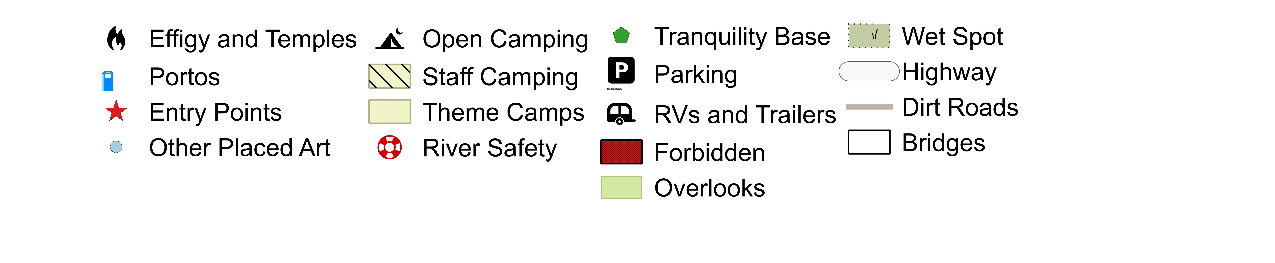
\includegraphics[width=\textwidth]{images/Legend}
% \begin{multicols}{3}
% \begin{itemize}
% \item[] 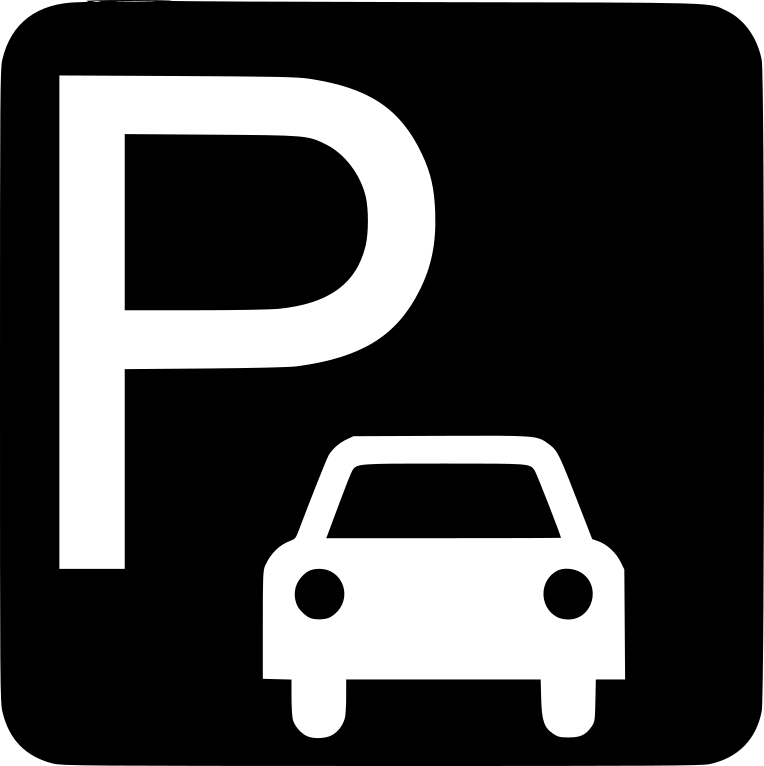
\includegraphics[height=8mm]{images/parking} \quad Parking
% \item[] 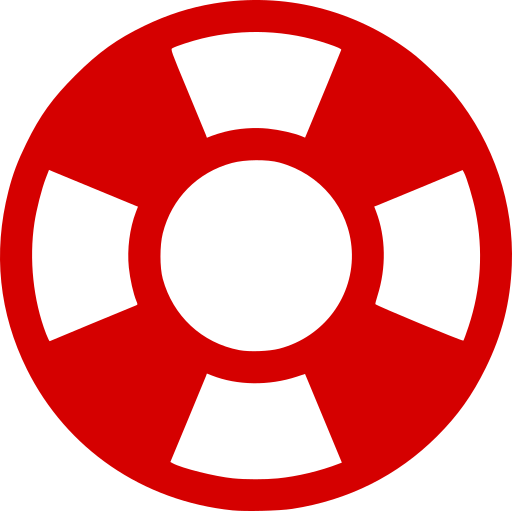
\includegraphics[height=8mm]{images/lifesaver} \quad \parbox[t]{\linewidth-\widthof{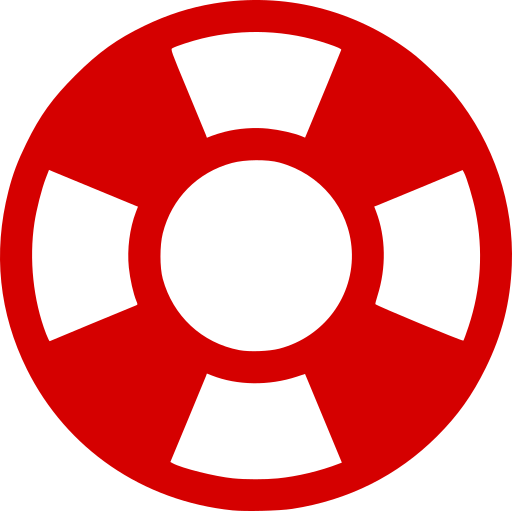
\includegraphics[height=8mm]{images/lifesaver}}}{River Safety\\ Equipment}
% \item[] 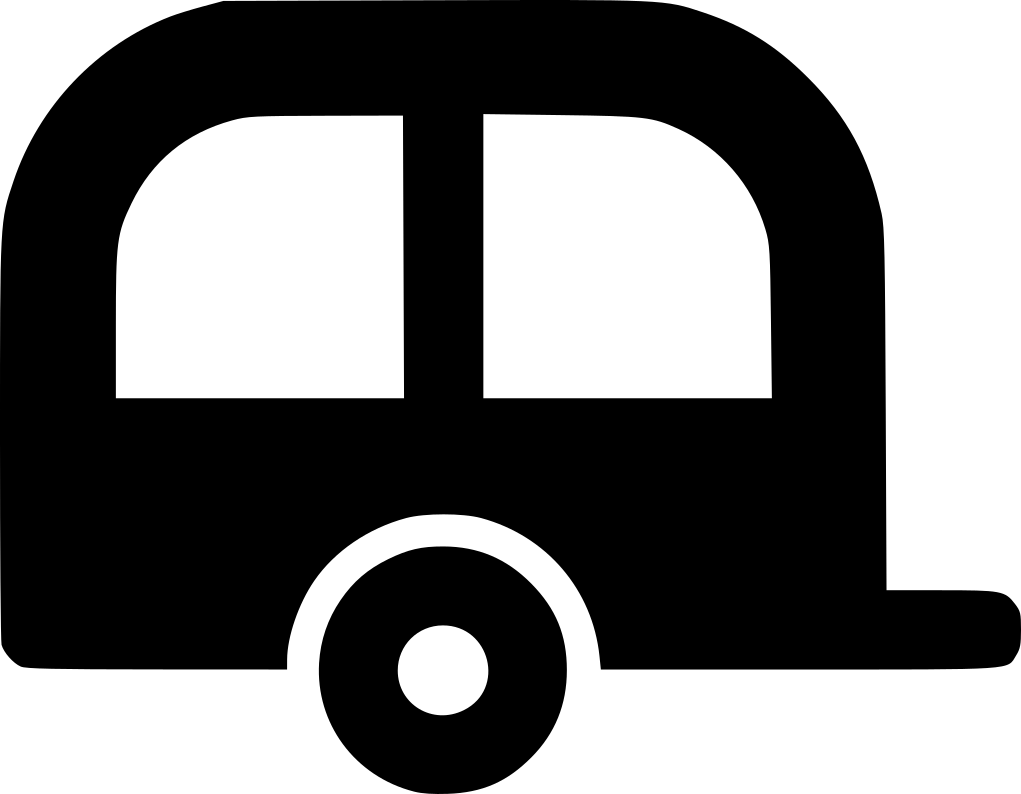
\includegraphics[height=8mm]{images/camper} \quad RV Camping
% \item[] 
\includegraphics[height=8mm]{images/camping} \quad Open Camping
% \item[] 
\includegraphics[height=8mm]{images/portapotty} \quad Port-a-Potty
% \end{itemize}

% \end{multicols}

% \begin{tabular}{llllll}
% 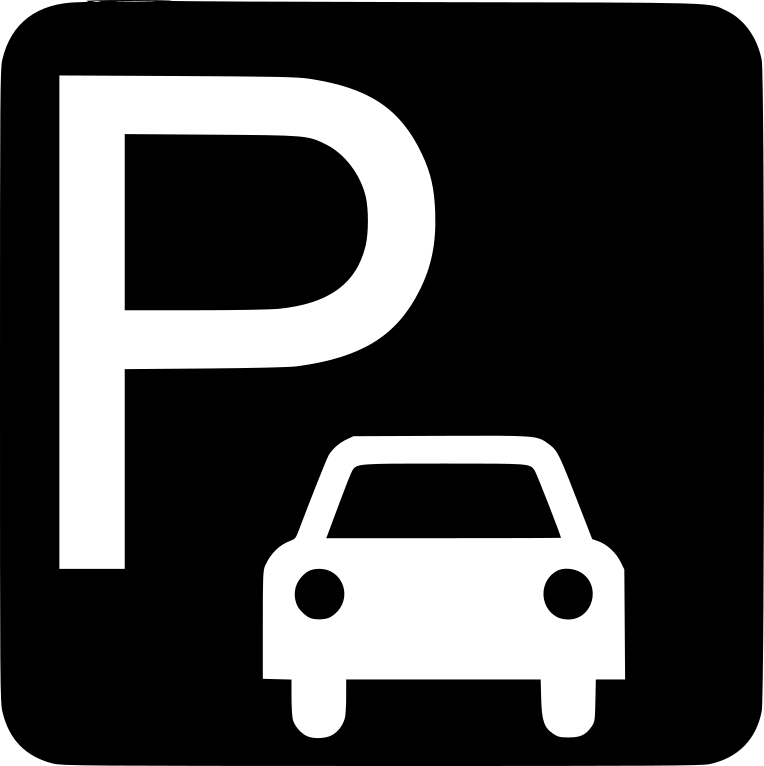
\includegraphics[height=8mm]{images/parking} & Parking & 
% 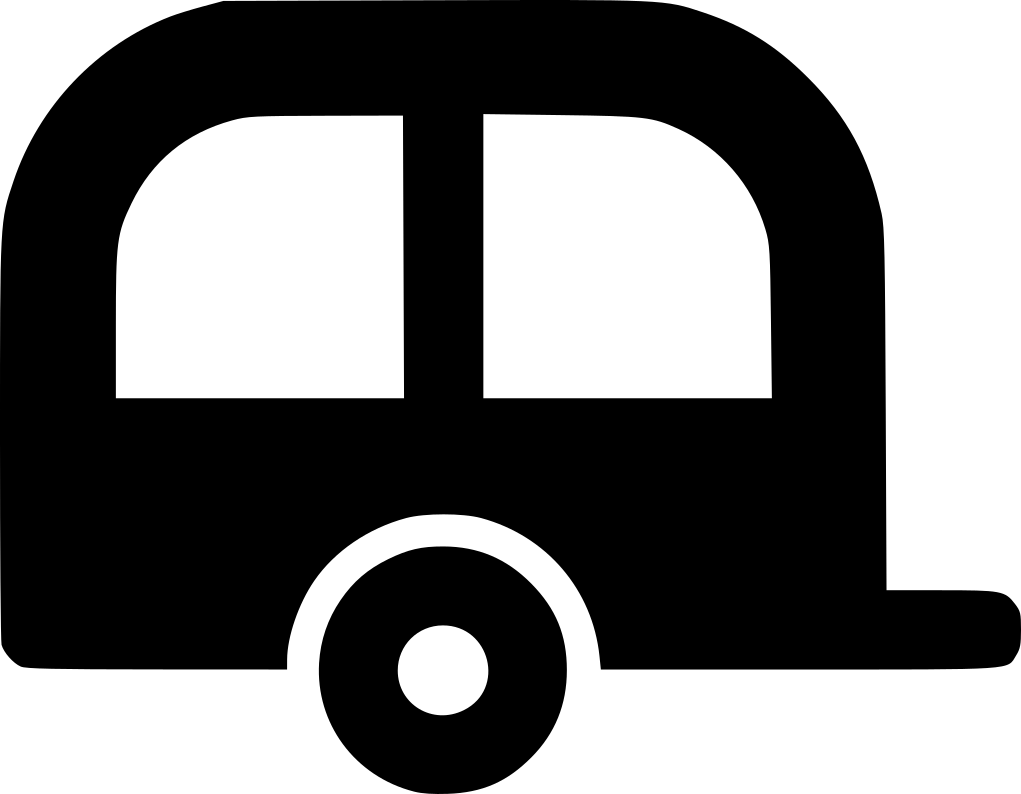
\includegraphics[height=8mm]{images/camper} & RV Camping & 
% 
\includegraphics[height=8mm]{images/portapotty} & Port-a-Potty \\
% 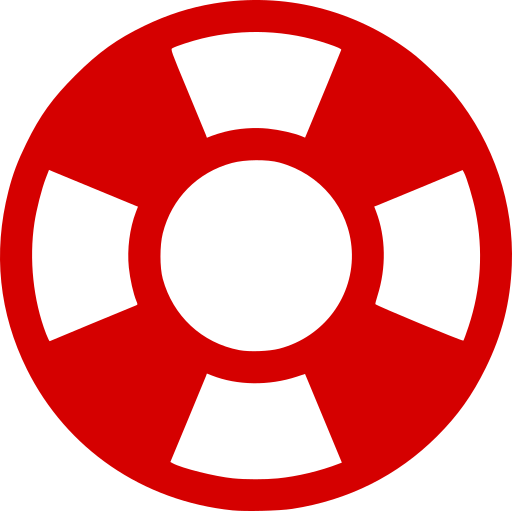
\includegraphics[height=8mm]{images/lifesaver} & \parbox[t]{3cm}{River Safety \\Equipment} & 
% 
\includegraphics[height=8mm]{images/camping} & Open Camping  
% &  & 
% \end{tabular}

\vspace*{\fill}
\begin{center}
	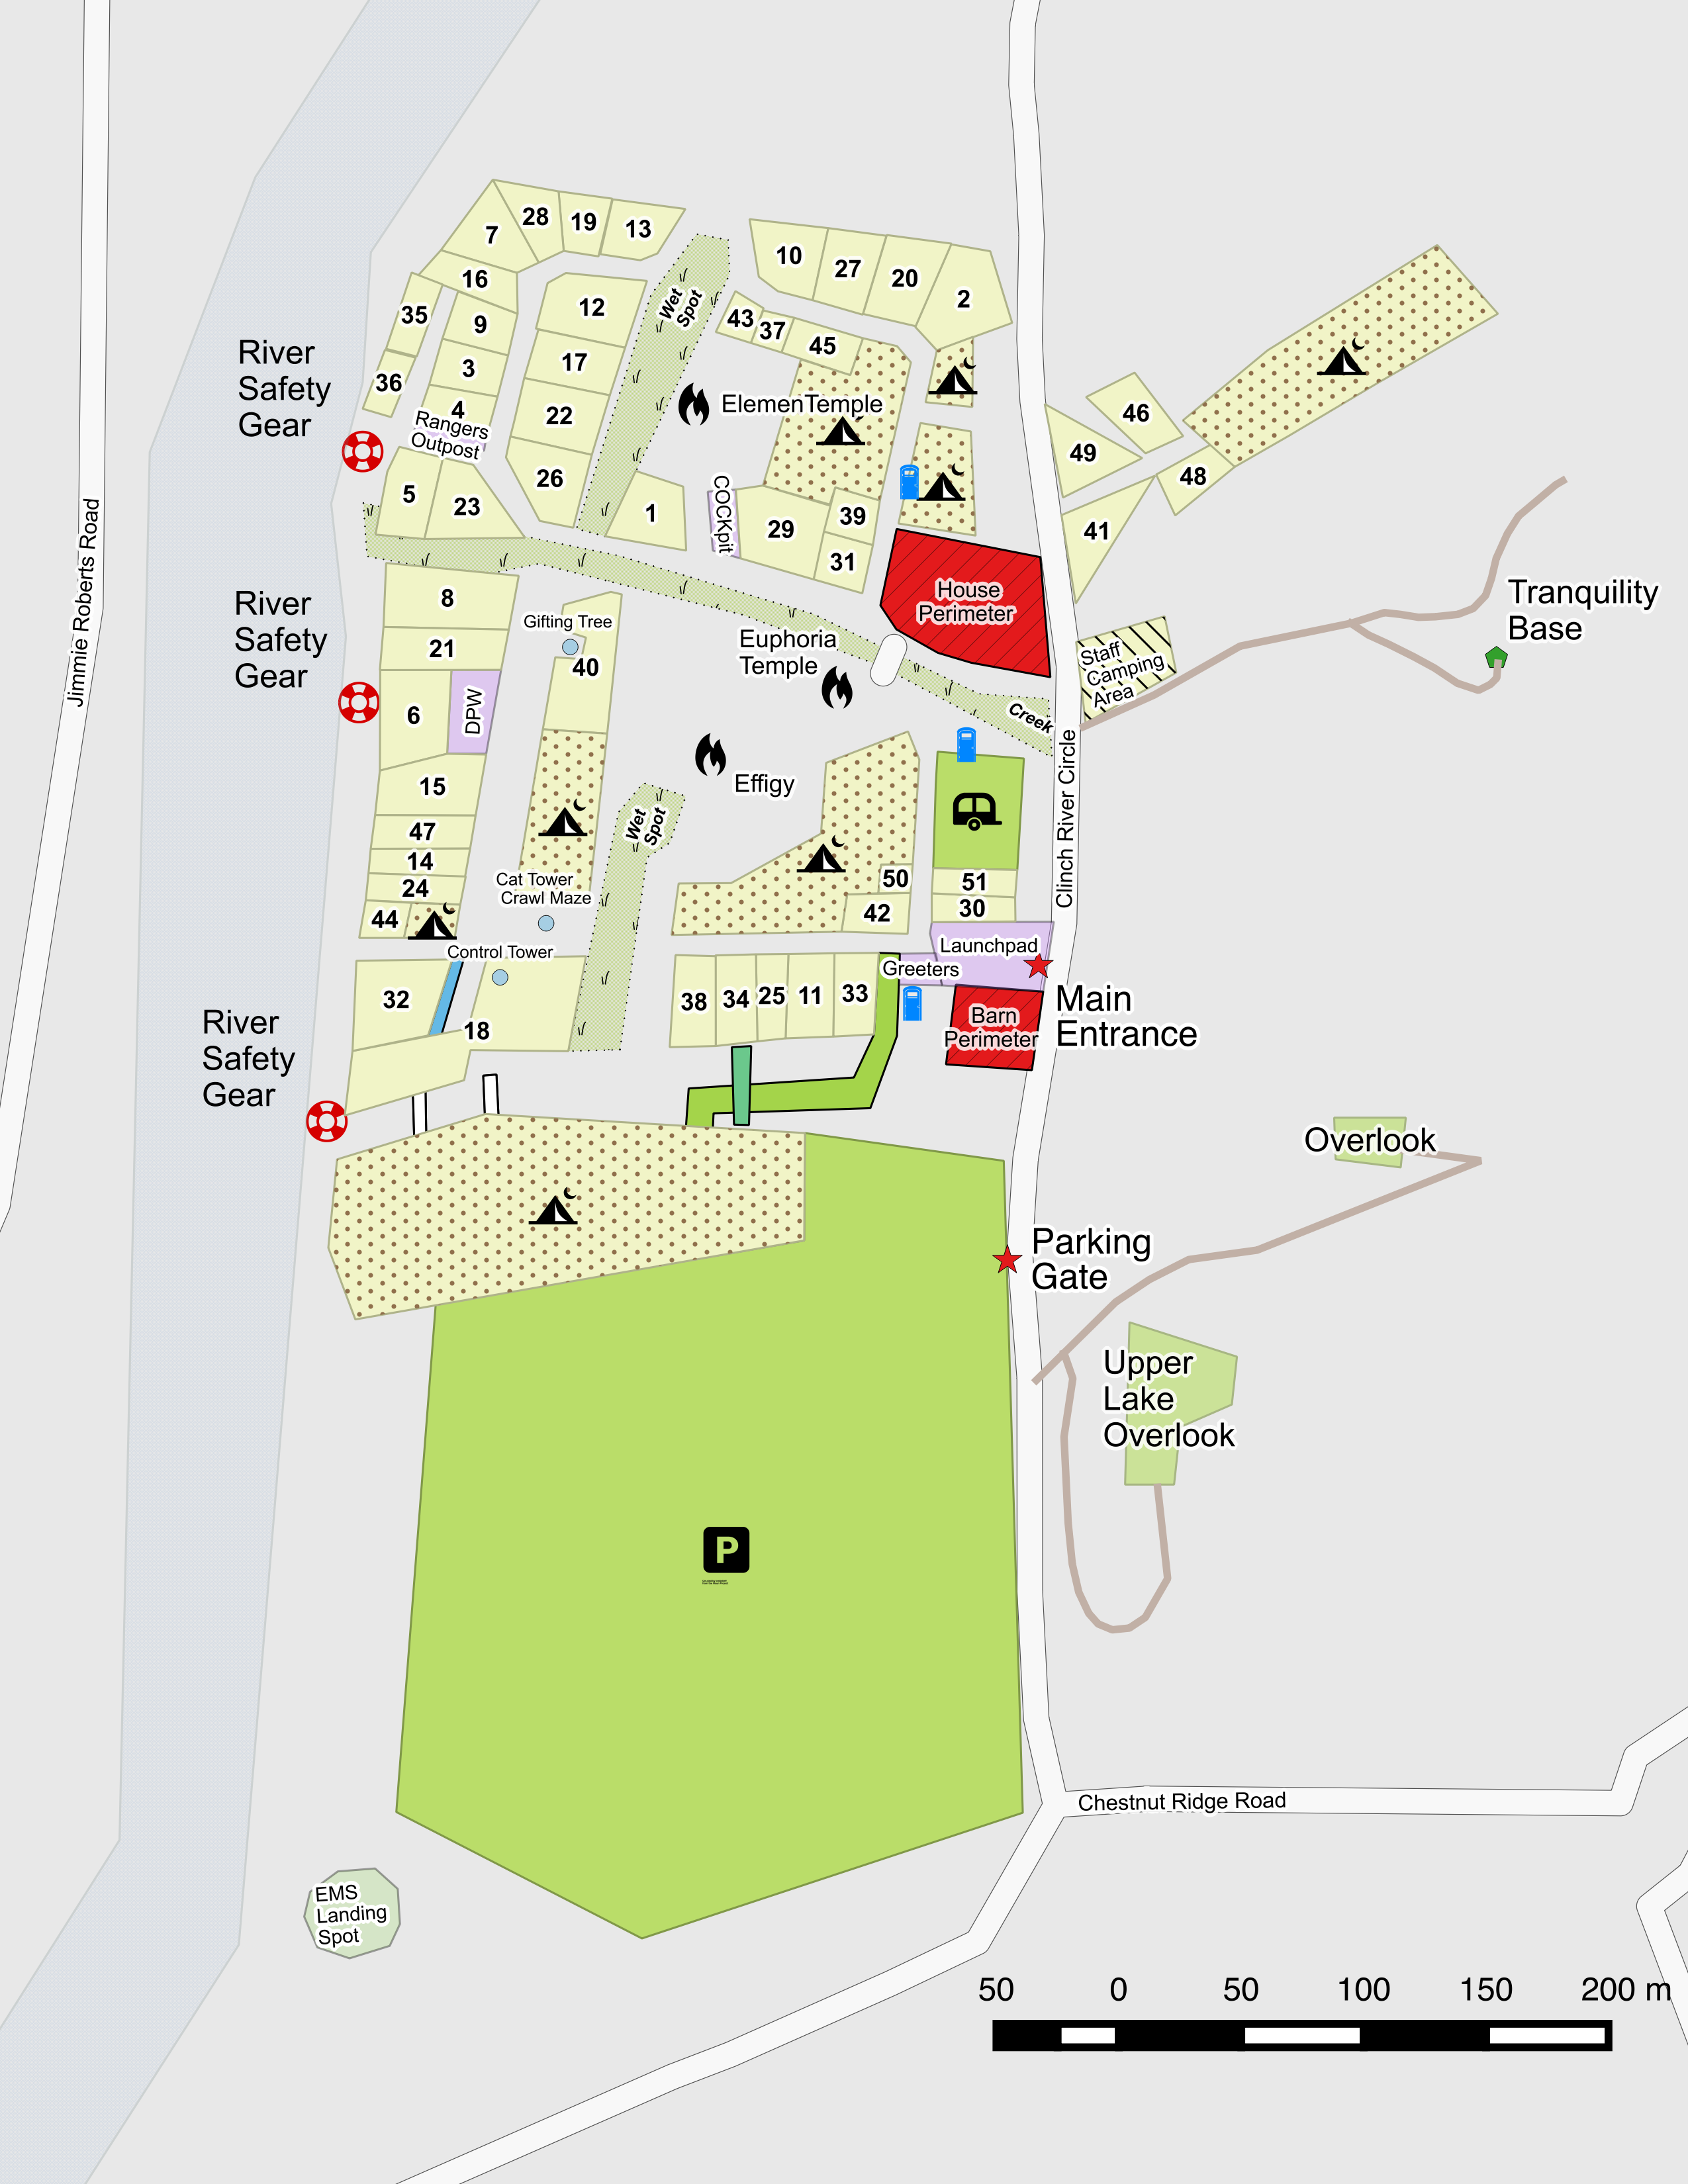
\includegraphics[width=.95\textwidth]{images/TTM2018}
\end{center}
\vspace*{\fill}

% We want this to be the back cover
\clearpage
\thispagestyle{empty}
\begin{figure}[h!]
	\centering
	
\includegraphics[angle=90,width=\textwidth]{images/TTM2018_smaller}
    \small
    (Artwork courtesy Thomas O'Connor)
\end{figure}

\end{document}
